
% Cal Poly Thesis
% 
% based on UC Thesis format
%
% modified by Mark Barry 2/07.
%




\documentclass[12pt]{ucthesis}

%\newif\ifpdf
%\ifx\pdfoutput\undefined
%    \pdffalse % we are not running PDFLaTeX
%\else
%\pdfoutput=1 % we are running PDFLaTeX
%\pdftrue \fi

\usepackage{textcomp}
\usepackage{url}
\usepackage{float}
\usepackage[usenames,dvipsnames]{color}
\usepackage{listings}
\lstset{
    language=C++,
    basicstyle=\small\ttfamily\bfseries,
    frame=tb,
    numbers=left,
    numberstyle=\tiny,
    numbersep=-4pt,
    columns=fullflexible,
    showstringspaces=false,
    captionpos=b,
    keywordstyle=\color{Blue},
    morekeywords={function,local,then,end},
    commentstyle=\color{OliveGreen},
    stringstyle=\color{BrickRed}
}
\usepackage{color}
%\ifpdf

    \usepackage[pdftex]{graphicx}
    % Update title and author below...
    \usepackage[pdftex,plainpages=false,breaklinks=true,colorlinks=true,urlcolor=blue,citecolor=blue,%
                                       linkcolor=blue,bookmarks=true,bookmarksopen=true,%
                                       bookmarksopenlevel=3,pdfstartview=FitV,
                                       pdfauthor=Robert Edward Somers,
                                       pdftitle=FlexRender: A distributed rendering architecture for ray tracing huge scenes on commodity hardware.,
                                       pdfkeywords={thesis, masters, cal poly, ray tracing, distributed rendering}
                                       ]{hyperref}
    %Options with pdfstartview are FitV, FitB and FitH
    \pdfcompresslevel=1

%\else
%    \usepackage{graphicx}
%\fi

\usepackage{amssymb}
\usepackage{amsmath}
\usepackage[letterpaper]{geometry}
\usepackage[overload]{textcase}



%%%%%\bibliographystyle{abbrv}

\setlength{\parindent}{0.25in} \setlength{\parskip}{6pt}

\geometry{verbose,nohead,tmargin=1.25in,bmargin=1in,lmargin=1.5in,rmargin=1.3in}

\setcounter{tocdepth}{2}


% Different font in captions (single-spaced, bold) ------------
\newcommand{\captionfonts}{\small\bf\ssp}

\makeatletter  % Allow the use of @ in command names
\long\def\@makecaption#1#2{%
  \vskip\abovecaptionskip
  \sbox\@tempboxa{{\captionfonts #1: #2}}%
  \ifdim \wd\@tempboxa >\hsize
    {\captionfonts #1: #2\par}
  \else
    \hbox to\hsize{\hfil\box\@tempboxa\hfil}%
  \fi
  \vskip\belowcaptionskip}
\makeatother   % Cancel the effect of \makeatletter
% ---------------------------------------

\begin{document}

% Declarations for Front Matter

% Update fields below!
\title{FlexRender: A distributed rendering architecture for ray tracing huge
scenes on commodity hardware.}
\author{Robert Edward Somers}
\degreemonth{June} \degreeyear{2012} \degree{Master of Science}
\defensemonth{June} \defenseyear{2012}
\numberofmembers{3} \chair{Zo\"{e} Wood, Ph.D.} \othermemberA{Chris Lupo, Ph.D.} \othermemberB{Phillip Nico, Ph.D.} \field{Computer Science} \campus{San Luis Obispo}
\copyrightyears{seven}



\maketitle

\begin{frontmatter}

% Custom made for Cal Poly (by Mark Barry, modified by Andrew Tsui).
\copyrightpage

% Custom made for Cal Poly (by Andrew Tsui).
\committeemembershippage

\begin{abstract}

As the quest for more realistic computer graphics marches steadily on, the
demand for rich and detailed imagery is greater than ever. Unfortunately, our
appetite for large and complex geometry is quickly outpacing advances in the
hardware used to render it. Scenes with hundreds of millions or even billions
of polygons are not only desired, they are demanded.

Techniques such as normal mapping and level of detail have attempted to address
the problem by reducing the amount of geometry in a scene. This is problematic
for applications that desire or demand access to the scene's full geometric
complexity at render time. More recently, out-of-core techniques have provided
methods for rendering large scenes when the working set is larger than the
available system memory.

We propose a distributed rendering architecture based on message-passing that
is designed to partition scene geometry across a cluster of commodity machines
in a spatially coherent way, allowing the entire scene to remain in-core and
enabling the construction of hierarchical spatial acceleration structures in
parallel. The results of our implementation show over an order of magnitude
speedup in rendering time compared the traditional approach, while keeping
memory overhead for message queuing around 1\%.

\textbf{TODO: motivate commodidy machines (price/performance ratio, you already have it, etc.}

\textbf{TODO: bring claims in line with results}

\end{abstract}

%\begin{acknowledgements}

%   Thank you...

%\end{acknowledgements}


\tableofcontents


\listoftables

\listoffigures

\end{frontmatter}

\pagestyle{plain}




\renewcommand{\baselinestretch}{1.66}


% ------------- Main chapters here --------------------





\chapter{Introduction}
\label{intro}

\emph{Rendering}, the process of taking the description of a scene and turning
it into a visual image, has advanced at an incredible pace in recent
years. Many techniques have been developed to turn these descriptions into
pixels, and countless more have targeted weaknesses or challenges with those
algorithms. As the field continues to evolve and grow, new algorithms will be
born, others will fall out of favor and die, and some will soldier on. Only
one thing remains constant: The desire to bring our computational models ever
closer to mimicking physical reality.

\section{Geometric Complexity}
\label{complexity}

At the heart of mimicking reality is describing the world we wish to show. In
computer graphics, this has traditionally been done by defining surfaces. While
exciting developments in volume rendering techniques happen on regular basis,
it is unlikely we will abandon using surfaces any time soon. Unfortunately for
volumes, they are inherently an $n^3$ problem (where $n$ is the size of the
volume in one dimension) and $n^3$ is not a particularly friendly number in the
field of Computer Science.

For now and the foreseeable future, it seems, surfaces will be our bread and
butter. Many methods have been developed for describing surfaces to computer
programs, such as level sets, implicitly defined surfaces from mathematical
equations, and curvilinear forms such as parametric splines. The undisputed
champion of surface representations, however, has been the polygonal mesh.
Countless man-years of research and development has yielded efficient
techniques for processing meshes of interconnected polygons at blistering
speeds, and many other surface representations are ultimately converted to a
polygonal mesh at some stage of the rendering pipeline.

Meshes are easy for artists to work with because they represent discrete
points in space and the connectivity between those points (rather than abstract
equations). However, their core advantage is also their core drawback. Because
everything is defined explicitly, meshes with fine levels of detail have
significantly higher storage requirements. Thus, as the demand for higher
visual fidelity increases, the natural tendency is to increase geometric
complexity.

\section{Parallel Rendering}
\label{parallel}

Graphics has long been said to be a problem that is \emph{embarrassingly parallel},
given that many graphics algorithms operate on pixels independently. Graphics
processing units (GPUs) have exploited this fact for many years to achieve
amazing throughput of graphics primitives in real-time. Ray tracing in
particular (discussed more thoroughly in Section \ref{raytracing}) is commonly
paraded as the poster child for parallel processing.

Unfortunately the story is not all unicorns and rainbows. While processor
architectures have become exceedingly parallel and posted impressive
speedups, the memory hierarchy has not had time to catch up. For a processor
to perform well, the CPI, \emph{cycles per instruction}, must remain low to
ensure time is spent doing useful work and not waiting on data.

In current memory hierarchies, data access time can take anywhere from around
12 cycles (4 nanoseconds for an L1 cache hit) to over 300 cycles (100
nanoseconds for main memory). Techniques such as out-of-order execution are
helpful in filling this wasted time, but for memory intensive applications it
can be difficult to fill all the gaps with useful work. Thus, keeping the chips
"hot" by reducing time spent waiting on data is critical to achieve maximum
performance, and is an extremely challenging problem.

\begin{figure}[h!]
    \centering
    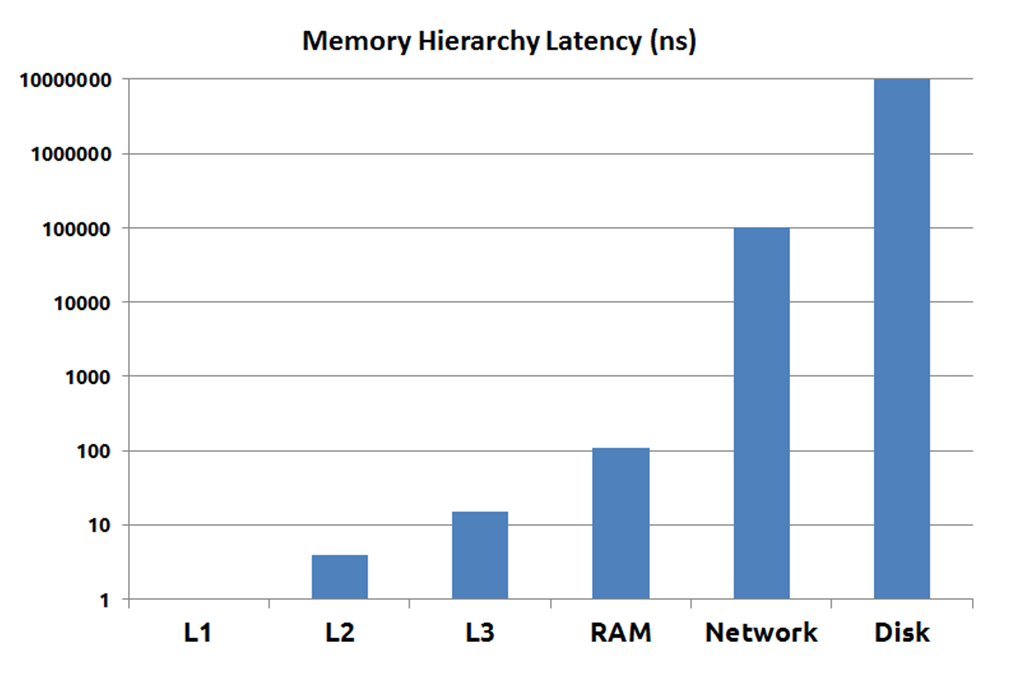
\includegraphics[width=140mm]{figures/memorylatency.png}
    \captionfonts
    \caption{Typical memory latencies in a modern commodity machine. Gigabit ethernet latency included for comparison.}
    \label{fig:memlatency}
\end{figure}

Because of this fact, there is a lot more to parallel rendering than initially
meets the eye. Graphics may indeed by highly parallel, but its voracious appetite
for memory access is actively working \emph{against} its parallel efficiency on
current architectures.

\section{Our Contribution}
\label{contribution}

This paper presents the architecture of FlexRender, a ray tracer designed for
rendering huge scenes with high geometric complexity on commodity hardware. We
specifically target commodity hardware because it currently has an excellent
cost to performance ratio, but still typically lacks enough memory to fit large
scenes entirely in RAM.

Current strategies for parallelizing a renderer across a cluster of commodity
machines are limited to having each worker compute a separate ``slice" of the
image, but do nothing to manage the high cost associated with large scene
assets.

Thus, our work describes the following core contributions:

\begin{enumerate}
    \item A system for ray tracing which uses the pooled memory of a cluster of
        commodity machines to keep the entire scene in-core.
    \item A method for passing ray messages between workers in the cluster with
        enough state to never require a reply message.
    \item An extension to the stackless BVH traversal algorithm presented by
        Hapala et al. \cite{hapala:2011} that makes it possible to suspend
        traversal at one worker and resume it at another.
    \item A discussion of the concepts involved and an analysis of the resulting
        implementation.
\end{enumerate}

In particular, we show that FlexRender can achieve speedups that exceed an
order of magnitude over the traditional parallelization approach, and can
naturally self-regulate the cluster of workers to keep the memory overhead due
to message queuing around 1\% of each worker's system memory.

\textbf{TODO: bring claims in line with results}

\chapter{Background}
\label{background}

The FlexRender architecture builds on the four fundamental building blocks
described here. First, we discuss the linearity of light (Section \ref{radiometry}),
which is critical to understanding why FlexRender produces a correct composite
image from pieces rendered by different workers. Next, we give a general
overview of ray tracing (Section \ref{raytracing}) and bounding volume hierarchies
(Section \ref{bvhs}). Finally, we discuss Morton coding and the Z-order curve
(Section \ref{morton}) which FlexRender uses to distribute scene data amongst the
workers.

\section{Light and Radiometry}
\label{radiometry}

\emph{Radiometry}, the study of propagation of electromagnetic radiation, forms
the basis for many rendering algorithms. Our coverage will be brief, but we will
examine some critical theory that enables the design of FlexRender. For a more
complete treatment of the topic in the context of rendering algorithms, we refer
the reader to \emph{Physically Based Rendering} \cite{pbrt}.

At its core, radiometry is based on modeling light as radiant energy and
operates at the level of geometric optics. In other words, we acknowledge that
light has wave-like properties and visible light occurs within a spectrum of
wavelengths (roughly 400 to 750 nm), but we do not mathematically model it as
a wave. Rather, we model it as a particle of radiant energy. In ray tracers
(discussed in depth in Section \ref{raytracing}) we model the path traveled by a single
particle of light with a ray.

The interesting parts of the radiometry model with respect to FlexRender are the
following observations:

\begin{description}
    \item[Light behaves linearly.] The combined effect of two rays of light
        in a scene is the same as the sum of their independent effects on the
        scene.
    \item[Energy is conserved.] When a ray reflects off of a surface, it can
        never do so with more energy than it started with.
\end{description}

In particular, these assumptions allow us to make the following key
observations, which FlexRender explicitly exploits:

\begin{description}
    \item[The location of computation does not matter.] If the scene is
        distributed across many workers, it makes no difference which worker
        computes the effect of a ray. The sum of all the workers' computations
        will be the same as if all the work was performed on a single worker.
    \item[Transmittance models energy conservation.] If we store the amount of
        energy traveling along a ray (the \emph{transmittance}) with the ray
        itself, we need not know anything about the preceding rays or state
        that brought this ray into existence. We can compute its contribution
        to the scene independently and ensure that linearity and energy
        conservation are both respected.
\end{description}

\section{Ray Tracing}
\label{raytracing}

\emph{Ray tracing} is a method for rendering a scene from some input description.
The ray casting algorithm, published by Appel in 1968 \cite{appel:1968}, proposed
shooting rays out of the camera and computing their intersections with mathematically
defined surfaces. One ray is shot through the center of every pixel, and the first
object that ray intersects is what is seen through the camera at the pixel.

\begin{figure}[h!]
    \centering
    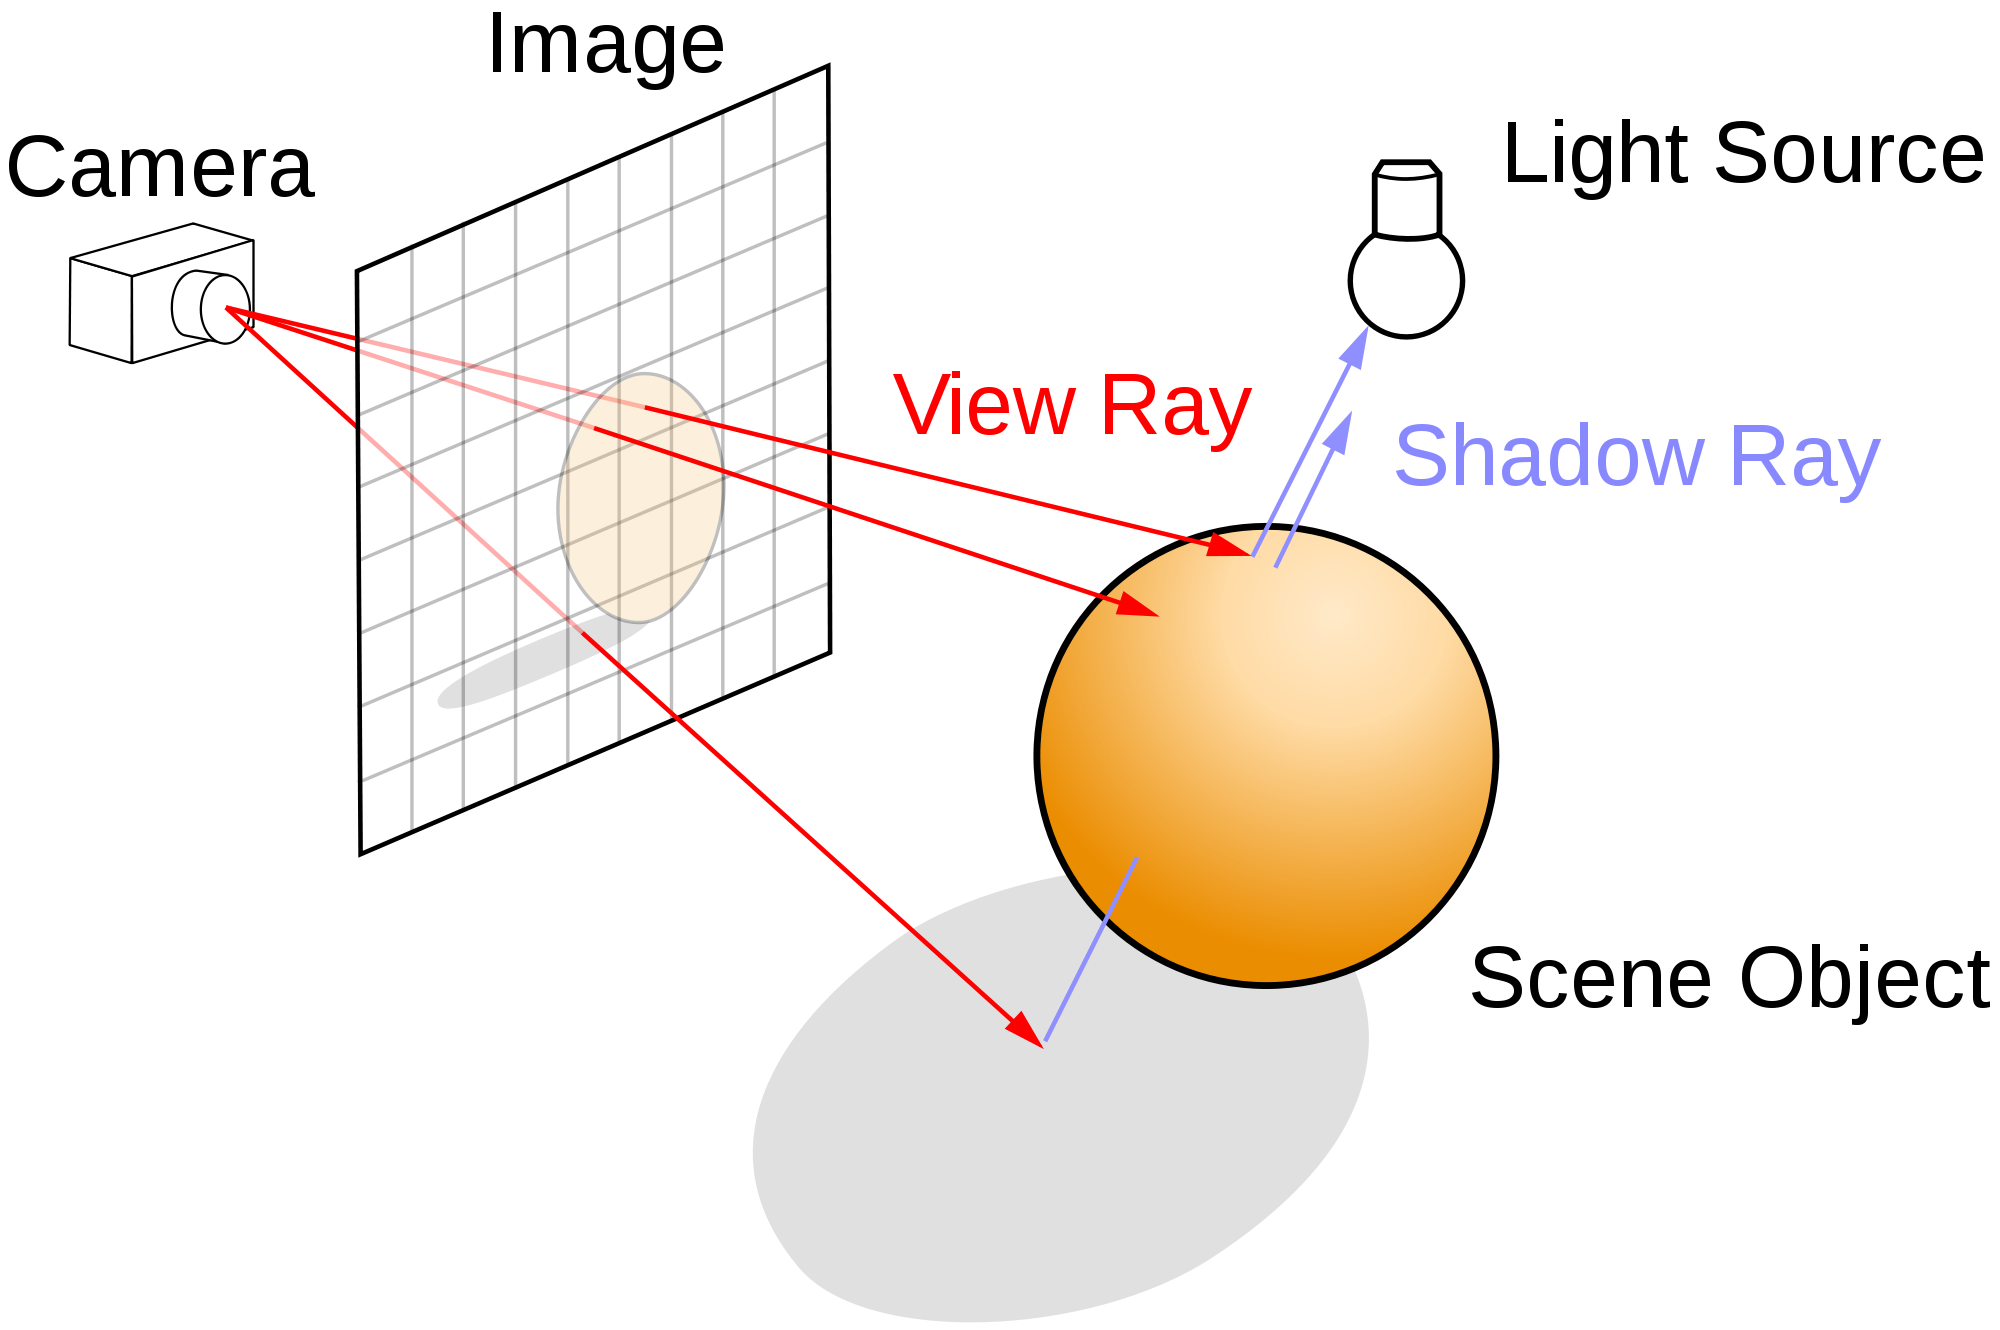
\includegraphics[width=110mm]{figures/raytracing.png}
    \captionfonts
    \caption{Ray tracing models light by shooting rays into the scene from the camera. Credit: ``Henrik" (Creative Commons License)}
    \label{fig:raytracing}
\end{figure}

In 1980, Whitted published an extention of this idea \cite{whitted:1980},
which continued the process at the point of intersection. At that point a shadow
ray is cast from the intersection point to the light to determine if the
point is illuminated or in shadow. He also introduced the notion of tracing
rays recursively, casting new rays into the scene, originating at the intersection
point, whose directions are computed by reflecting or refracting them about the
surface normal at the point of intersection.

\begin{figure}[h!]
    \centering
    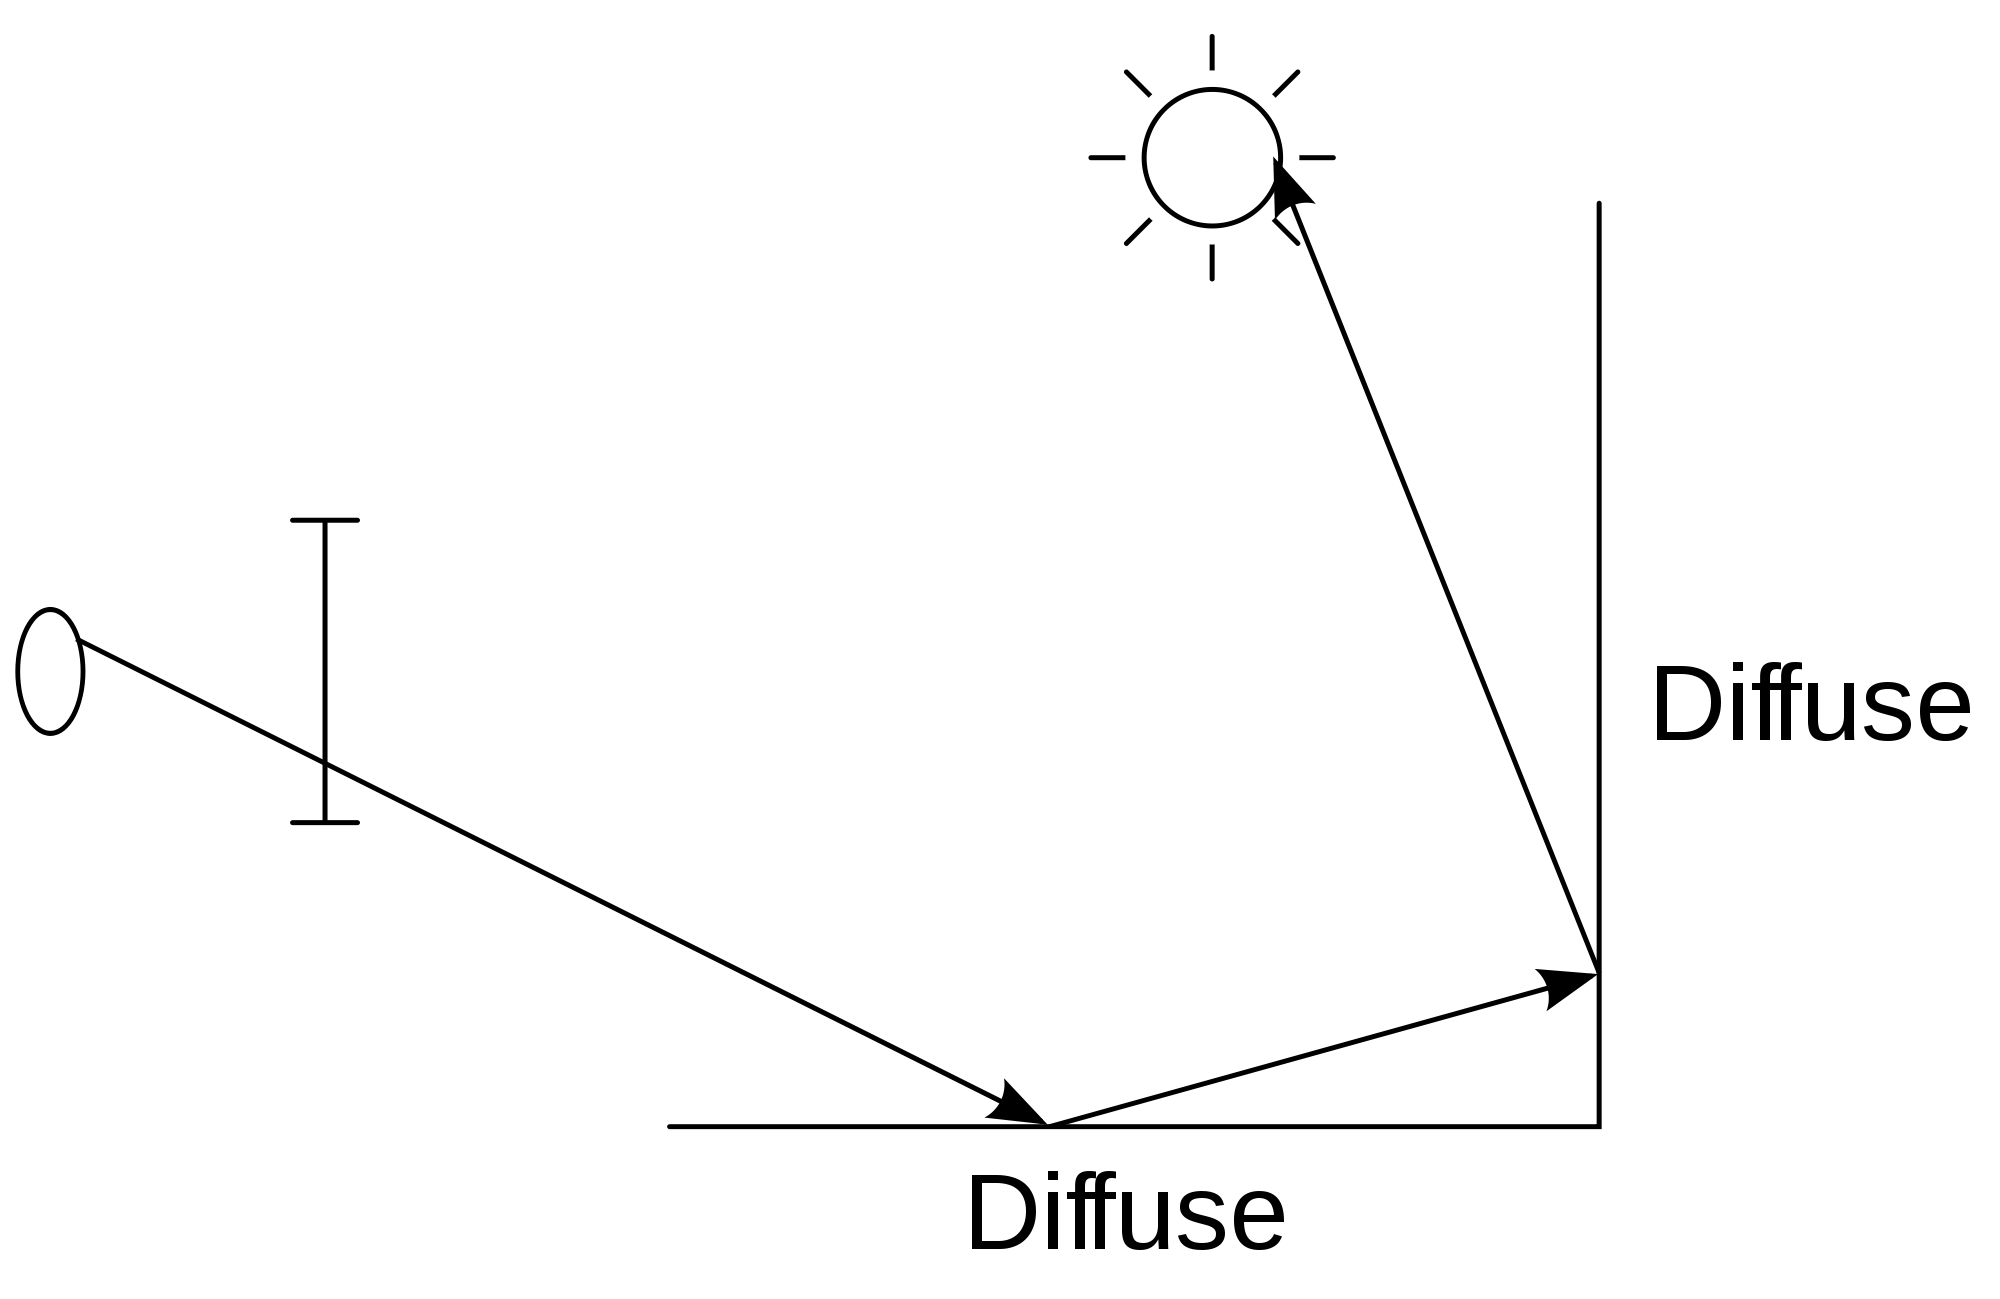
\includegraphics[width=90mm]{figures/reflectionrefraction.png}
    \captionfonts
    \caption{Reflection and refraction are modeled by casting new rays from intersection points. Credit: ``Stannered" (Creative Commons License)}
    \label{fig:reflectrefract}
\end{figure}

Ray tracing has significant advantages over other rendering algorithms (such
as scanline rasterization) because of it more closely models the way light acts
in the real world. Effects that are difficult to simulate using other methods
(such as shadows and correct reflections) fall out of the the algorithm naturally,
making it an attractive choice.

However, it suffers from performance problems. Without a method for reducing
the number of intersection tests in a scene, each ray must be tested against
every object, leading to $O(n)$ performance. Since rays are cast for each pixel
in the image (or multiple rays per pixel if stratified supersampling is used
for antialiasing) the number of rays scales with the resolution of the output
image.

Lastly, to approximate shadows with soft edges and other subtle lighting effects,
Monte Carlo integration is typically used when casting the shadow rays to the light.
This means that for every intersection, $n$ sample points are computed on the surface
of the light and a shadow ray is cast from the intersection point to each sample
point. The results of those casts are weighted by $\frac{1}{n}$ when computing the
shaded value at a point. Reflection and refraction also increase the number of
rays in play. To compute global illumination (the effect of light reflecting off
of all surfaces in the scene), the ray count increases dramatically.

Although it is common to see an exponential explosion of rays, thankfully we
have algorithms for significantly reducing the number of intersection tests we
need to compute per ray, which we will discuss in Section \ref{bvhs}.

\section{Bounding Volume Hierarchies}
\label{bvhs}

Bounding volume hierarchies, or BVHs, are essentially an application of binary
search to 3D space. In ray tracing, the vast majority of time is spent
computing intersection tests to determine whether a ray intersects a given
primitive. BVHs allow us to search 3D space for a potential intersection in a
binary tree fashion, pruning off large numbers of primitives with a single
test. Since it is effectively binary search, it is unsurprising that it reduces
intersection searching from linear time $O(n)$ to logarithmic time $O(log\;n)$
(assuming the BVH is well formed).

\begin{figure}[h!]
    \centering
    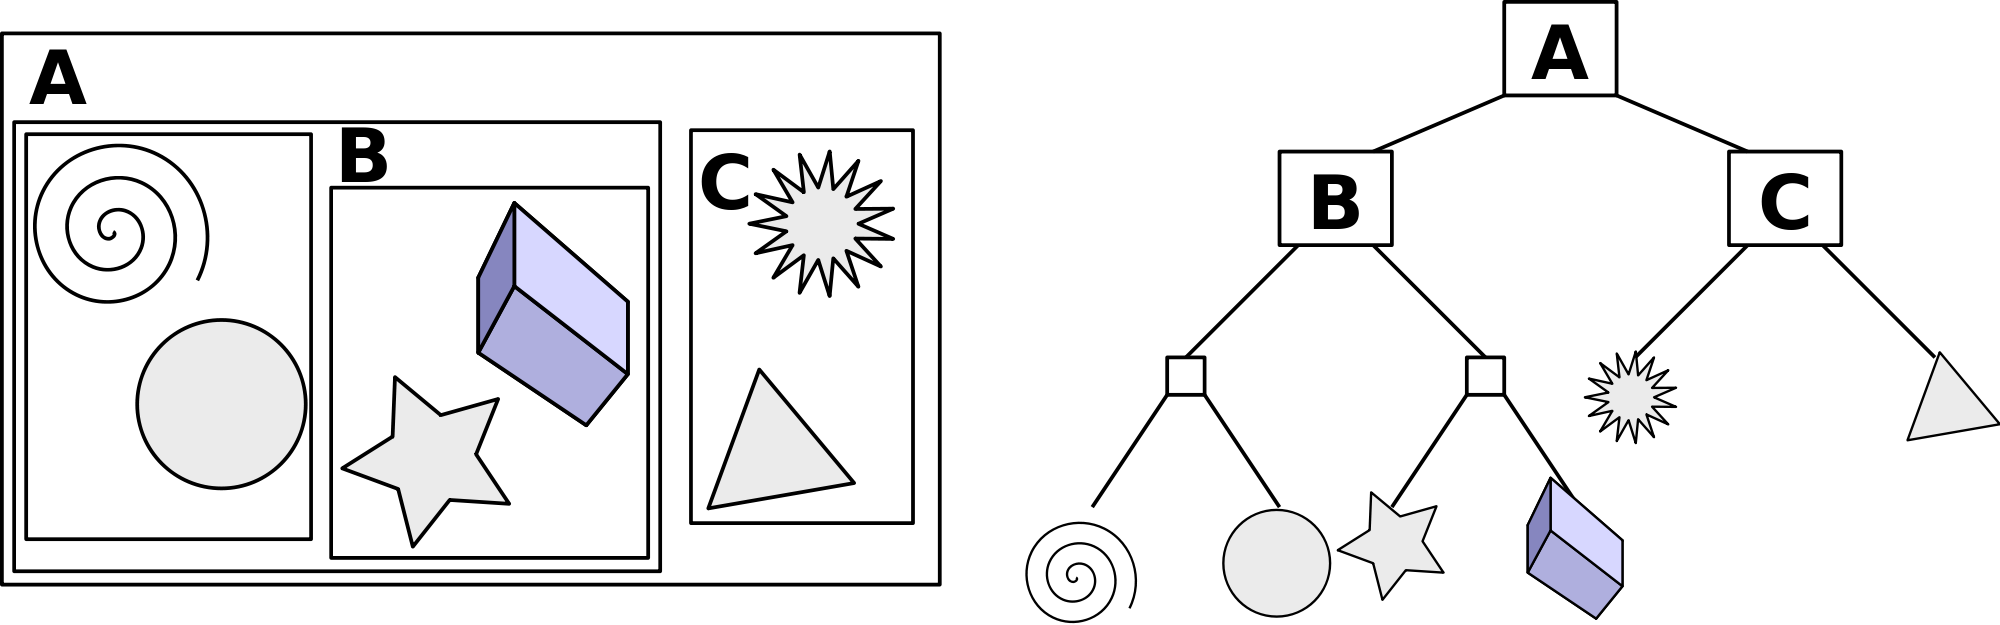
\includegraphics[width=140mm]{figures/bvh.png}
    \captionfonts
    \caption{Bounding volume hierarchies partition primitives into a binary tree structure. Credit: ``Schreiberx" (Creative Commons License)}
    \label{fig:bvh}
\end{figure}

BVHs are trees where each node is defined by a bounding volume, such as a box
or a sphere, that describes the extents of a region of 3D space. All of the
primitives in the scene that are within that region of space are child nodes
in the tree. Each node has two direct children, which also define bounding
volumes within that subregion of space. Nodes which have other bounding volume
nodes as their children are \emph{interior} nodes. \emph{Leaf} nodes in the tree
define a bounding volume around a single primitive.

After the tree structure is built using a typical linked-memory data structure,
it is flattened into a linear array of nodes for storage efficiency and better
cache performance. Flattening is done by walking the tree in a depth-first
traversal. This means that the left-hand child of the node at index $n$ is
located at index $n + 1$ in the array of nodes. Each node stores an offset
index to its right-hand child. Because the indices are relative to the array
and not the array's location in memory, they are safe to pass back and forth
between workers and require no address translation.

To traverse the tree looking for intersections, we begin by testing the root
node's bounding volume for an intersection. If the ray intersects the volume,
we recursively test each of the node's children. Once we hit a leaf node,
we perform an actual ray-primitive intersection test to determine if the ray
hits the primitive.

The traversal algorithm is naturally recursive, but recursive implementations
keep their state on the call stack. In FlexRender, we may need to suspend the
traversal on one worker and resume it on another, so we need all of the
traversal state explicitly exposed. Refactoring it as an iterative traversal
explicitly exposes the state for capturing.

The iterative algorithm still requires a traversal stack of child nodes that
need to be visited on the way back up the tree. Since this stack is unique for
each ray, the entire stack would need to be carried along with each ray. In
addition, the stack could potentially be large if the scene is huge (and thus,
the tree is deep), so it would be ideal if we had a method for traversing the
tree iteratively without the need to maintain a traversal stack.

A method for doing so is described by Hapala et al. in
\emph{Efficient Stack-less BVH Traversal for Ray Tracing} \cite{hapala:2011}.
Their key insight is that if parent links are stored in the tree, the same
traversal can be achieved using a three-state automaton describing the direction
you came from when you reached the current node (i.e. from the \emph{parent},
from the \emph{sibling}, or from the \emph{child}). They show that their
traversal algorithm produces identical tree walks and never retests nodes that
have already been tested.

FlexRender leverages this traversal algorithm due it its low state storage
requirements. Each ray only needs to know the index of the current node it is
traversing (in the array of flattened nodes) and the state of the traversal
automaton. The extensions made to the algorithm to support suspending traversal
and resuming it on another worker are described in Section \ref{traversal}.

\section{Morton Coding and the Z-Order Curve}
\label{morton}

Morton coding is a method for mapping coordinates in multidimensional space to
a single dimension. In particular, walking the multidimensional space with a
Morton coding produces a space-filling Z-order curve.

\begin{figure}[h!]
    \centering
    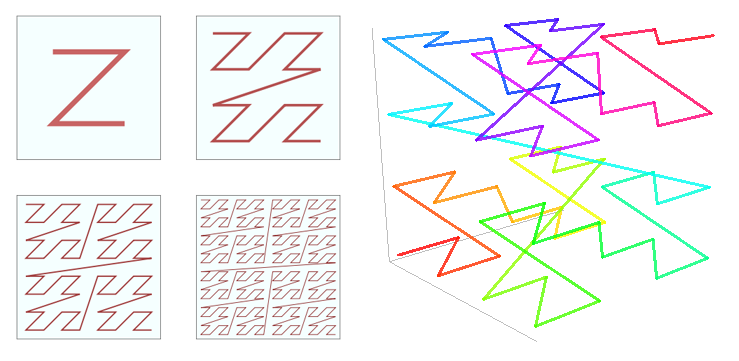
\includegraphics[width=110mm]{figures/zorder.png}
    \captionfonts
    \caption{Examples of two dimensional and three dimensional Z-order curves. Credit: ``David Eppstein" and ``Robert Dickau" (Creative Commons License)}
    \label{fig:zorder}
\end{figure}

More concretely, FlexRender needs a way to distribute a large scene to many
workers in a spatially coherent way. If the geometry on each worker consists
of a localized patch of the overall geometry, it allows us minimize communication
between the workers, and thus, only pay the network cost when we absolutely need
to (described in depth in Section \ref{traversal}).

Because the Morton coding produces a spatially coherent traversal of 3D space,
dividing up the 1D Morton code address space among all the workers participating
in the render gives a reasonable assurance of spatial locality for the geometry
sent to each worker.

The Morton coding is relatively simple to implement. For example, say that
we wish to map a point $P$ in a region of 3D space (defined by its bounding extents
$min$ and $max$) to a Morton coded 64-bit integer. Discretizing each axis evenly
allows for 21 bits per axis, yielding a 63-bit address space (and one unused bit
in the integer).

Computing the Morton code is simply a matter of calculating the 21-bit discretized
component of $P$ along each axis, then shifting the components from each axis
into the 64-bit integer one bit at a time in a round robin fashion, from the
most-significant to least-significant bit.

\begin{lstlisting}[caption=Example of computing the Morton code.,label=mortoncode]
    // Discretize each component based 21 bits per axis.
    int factor = 0x1 << 21;
    int discrete_x = ((point.x - min.x) / (max.x - min.x)) * factor;
    int discrete_y = ((point.y - min.y) / (max.y - min.y)) * factor;
    int discrete_z = ((point.z - min.z) / (max.z - min.z)) * factor;

    uint64_t morton = 0;
    for (int bit = 20; bit >= 0; bit--) {
        // Set the bitmask.
        int mask = 0x1 << bit;

        // Extract the next bit from each component.
        int bit_x = (discrete_x & mask) >> bit;
        int bit_y = (discrete_y & mask) >> bit;
        int bit_z = (discrete_z & mask) >> bit;

        // Make space on the right edge of the Morton code.
        morton = morton << 3;

        // Set the x/y/z components.
        morton |= ((bit_x << 2) | (bit_y << 1) | (bit_z << 0));
    }
\end{lstlisting}


\chapter{Related Work}
\label{relatedwork}

Finding ways to deal with huge geometry has been a common theme in Computer
Graphics for quite a while. Early techniques generally focused on faking
high detail through clever use of textures and model swapping, since the
hardware of the day simply wasn't capable of handling massive amounts of data.

More recently, techniques have focused around actually having the the full
geometry available, but acknowledging that it won't fit in main memory and
providing methods for efficiently caching data that is out-of-core.

We examine these workarounds in Section \ref{workarounds}, and provide a brief
overview of relevant work in parallel rendering in Section \ref{parallelbg}.
We specifically discuss the Kilauea renderer, which had similar ambitions as
FlexRender but is significantly different in several ways.

\section{Big Geometry Workarounds}
\label{workarounds}

\subsection{Normal Mapping}
\label{normalmaps}

Normal mapping is a technique for simulating high resolution detail on a mesh
during shading while using low resolution geometry. The idea of extracting
detail from a high resolution mesh was first proposed by Krishnamurthy and
Levoy in 1996 \cite{krishnamurthy:1996}, which fit displacement maps over
from non-uniform rational B-splines (NURBS).

\begin{figure}[h!]
    \centering
    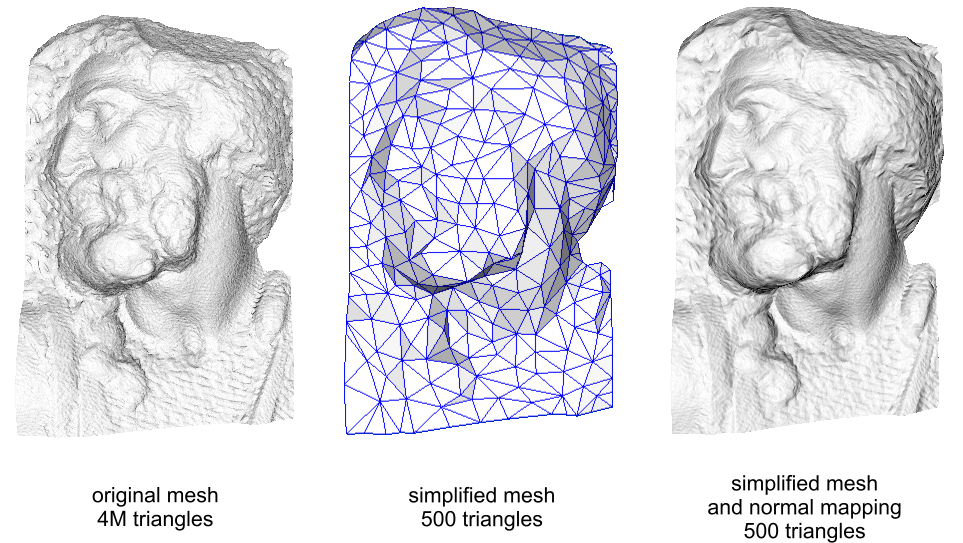
\includegraphics[width=100mm]{images/normalmapping.png}
    \captionfonts
    \caption{Normal mapping uses a texture to store high resolution shading normals on low resolution geometry.}
    \label{fig:normalmapping}
\end{figure}

Two additional papers completed the puzzle. In 1998 Cohen et al. \cite{cohen:1998}
presented a method for rendering high detail at shading time by storing normals
in the texture instead of using displacement maps, and Cignoni et at. \cite{cignoni:1998}
showed how this could be done with two meshes that were created independently.

Normal mapping is extensively used today, especially in real-time graphics
applications. However, it displays visual artifacts, particularly around the
edges of the mesh (where it's clearly apparent the surface is not high detail)
or areas where the texture is scrunched or streched.

\subsection{Level of Detail}
\label{levelofdetail}

Level of detail is a technique for replacing high resolution meshes with lower
resolution versions when they are some specified distance away from the viewer.
The idea was pioneered by James H. Clark in 1976 \cite{clark:1976}, when he
noticed that there was no reason to use high resolution geometry when the
resulting representation on the screen was tiny.

This technique is also still heavily used in real-time graphics applications
today. However it suffers from a few problems. The first is that multiple
resolutions of the mesh must be available. The second is that it is somewhat
depending on the size that the final image is viewed. A mesh may be small in
screen space compared to the size of the image, but on a movie-theater sized
screen it could very well still be quite large when viewed.

\subsection{Out-of-Core}
\label{outofcore}

Recent research have acknowledged that rendering data simply won't fit into
main memory any more, and have developed techniques for efficiently managing
a cache of rendering data in main memory. In 2011, Tabellion et al. \cite{tabellion:2011}
presented a technique for dealing with huge point clouds used in global
illumination. They showed that their method can process 88 GB of point cloud
data with a cache of just 2 GB, and can render 6.8 GB of point cloud data with
cache hit rates of over 99\%.

One year earlier, Pantaleoni et at. \cite{pantaleoni:2010} showed that their
software developed for Avatar also was very efficient at dealing with out-of-core
data. They used ray tracing to generate directional occlusion data, which was
compressed into spherical harmonics. The spherical harmonics were used at render
time (they did not directly ray trace the scenes during rendering). In particular,
they also used hierarchical BVHs with a single ``top-level" tree as FlexRender
does. However, they used it for chunking the scene into manageable units of work
that could be loaded and unloaded from main memory quickly.

\section{Parallel Rendering}
\label{parallelbg}

\subsection{Cooperative Networked Rendering}
\label{networked}

Without a doubt, the most similar piece of research to FlexRender is Kilauea
\cite{kato:2002}, a massively parallel networked renderer developed at Square
USA in 2002. Similarly to our work, it uses worker machines connected on a
network to keep the entire scene geometry in core. However, there are three
main differences in our approach.

\begin{description}
    \item[Geometry Distribution] \hfill \\
        Kilauea randomly distributes scene geometry to
        its workers, the casts intersections rays through all workers
        simultaneously. This may produce multiple candidate intersections. The
        results from each worker are gathered and a winner is picked using a
        standard depth test. This makes the pipeline highly senstive to extra
        latency on any of the workers, because everyone is waiting for the
        results to run the depth test.

        In contrast, FlexRender attempts to keep geometry spatially local among
        its workers. This allows us to build a hierarchical spatial acceleration
        structure over the workers and reduce the number of network hops we need
        to make to establish the correct intersection.
    \item[Shading Secondary Rays] \hfill \\
        When Kilauea decides to compute the shading value of a bounced ray, it
        suspends execution of the shader and keeps it around until the bounced
        ray comes back through the system. Similarly to FlexRender, they keep
        a priority queue for rays to process those most likely to terminate
        first.

        FlexRender maintains the source pixel and transmittance of each ray as
        state, so the suspension of shaders (and associated overhead) is
        unnecessary. Each worker has its own image buffer, which is composited
        into the final image at the end, respecting linearity.
    \item[Adaptability to Heterogeneous Architectures] \hfill \\
        Because Kilauea needs the results from every worker before performing
        the depth test, it is extremely latency sensitive. This encourages
        homogeneity among workers, and makes adding new workers into the cluster
        with vastly different machine architectures (such as GPGPU) or performance
        characteristics problematic.

        In contrast, workers in a FlexRender cluster are never waiting on
        the results from another worker. Thus, new machines can be dropped into the
        cluster without regard for how they will effect the latency of the entire
        system. For example, a GPGPU worker might batch up requests and outsource
        them to the GPU only when it can effectively amortize the cost of the
        memory bus transfer.
\end{description}

\subsection{General Purpose GPU Rendering}
\label{gpgpu}

As interest in General Purpose GPU, or GPGPU, computing has increased over
the last several years, many have decided to port ray tracers to the
architecture due to the problem's ``embarrassingly parallel" nature. Although
lots of simple implementations are floating around, only relatively recently
have researchers started tackling the challenging problems imposed by writing
a serious ray tracer on a GPGPU architecture device. It may be deceptively
straightforward to get a simple implementation up and running, but the
complexity is in the features and details required by a robust renderer.

Probably the most impressive recent work was done by Garanzha et al.
\cite{garanzha:2011:ray}, which presented a method for ray tracing large scenes that
are out-of-core on the GPU. Parts of their architecture are similar to FlexRender
on a single-device scale, specifically their use of multi-level BVHs for data that
is paged into memory and their use or ray queues to handle rays cast from shaders.
Their global ray queue, however, is fairly memory intensive, because it can
potentially store up to 32 million rays.

Another area of intense research has been spatial data structure construction
on the GPU. Although they usually produce data structures of slightly lower
quality than their CPU counterparts, these GPU algorithms go to great lengths
to produce ``high-enough" quality structures with dramatic speedups. Garanzha
et al. \cite{garanzha:2011:bvh} present a method for constructing BVHs on the
GPU and Wu et al. \cite{wu:2011} present a method for constructing KD-trees on
the GPU. Both are guided by the surface area heuristic.

\section{MapReduce}
\label{mapreduce}

Outside of the graphics world there has been great excitement surrounding
the MapReduce programming paradigm presented by Dean and Ghemawat in 2004
\cite{dean:2004}. For smaller scenes whose geometry and acceleration structure
data would fit entirely in-core on a single worker, this may be an interesting
approach worth exploring.

Northam and Smits \cite{northam:2011} presented a potential MapReduce
implementation of a ray tracer, but noted that sending large amounts of scene
data to the workers significantly slowed down scene processing. Their solution
was to break the scene into small chunks and resolve the winning intersection
test in the reduce step. While this works just fine, it also does a lot of
unnecessary work, because many non-winning intersections are computed that
would have been pruned in a typical BVH traversal.

\chapter{FlexRender Architecture}
\label{architecture}

In this chapter, we describe the network architecture and roles of the involved
machines in Section \ref{workers}. We discuss the structure of ray messages
passed between workers in Section \ref{fatrays} and briefly cover the design of
the graphics machinery shared between FlexRender and the baseline implementation
in Section \ref{types}. We detail the process of preparing the cluster for
rendering in Section \ref{sync} and Section \ref{parallelbvh}.

At its core, workers in the cluster are just ray processors. We discuss how they
manage ray messages in Section \ref{queues}, how they generate new work with
stable memory usage in Section \ref{primaryrays}, how we decide when and where
to send rays over the network in Section \ref{traversal}, and how shading is computed
when lights and occluders may exist anywhere in the cluster in Section \ref{illumination}.

Finally, we wrap up our discussion with how we monitor the progress of the
render in Section \ref{stats} and how we composite the final image from its
components in Section \ref{synthesis}.

\section{Organization and Design}
\label{organization}

\subsection{Workers and the Renderer}
\label{workers}

There are two potential roles a machine can play during the rendering process.

\begin{description}
    \item[Worker] These machines receive a chunk of the scene and act as ray
        processors to compute intersections and shading values. They produce
        an image that is a component of the final render. There may be an
        arbitrary number of them participating in a render.
    \item[Renderer] This machine reads in the scene data and distributes it to
        the workers. Once rendering begins it monitors the status of the each
        worker and halts any potential runaway situations (see Section \ref{primaryrays}).
        When the renderer decides the process is complete, it requests
        the image components from each worker and merges them into the final
        image. There is only a single renderer in any given cluster and it is
        the machine the user directly interacts with.
\end{description}

From a network perspective, the architecture is simply client/server connected
in a star topology. Each worker exposes a server which receives and
processes messages, and holds client connections open to every other worker for
passing messages around the cluster. The renderer also holds a client connection
to every worker for sending configuration data, preparing up the cluster for rendering
(described in Section \ref{sync}), and monitoring render progress (described in
Section \ref{stats}).

It is important to note that there is currently no fault tolerance built into
FlexRender. This decision was entirely due to limited resources and time
constraints; there is no architectural reason that the system could not be made
more robust and fault tolerant with the appropriate application of distributed
systems concepts. To that end, we refer the reader to the distributed systems
literature.

\begin{figure}[h!]
    \centering
    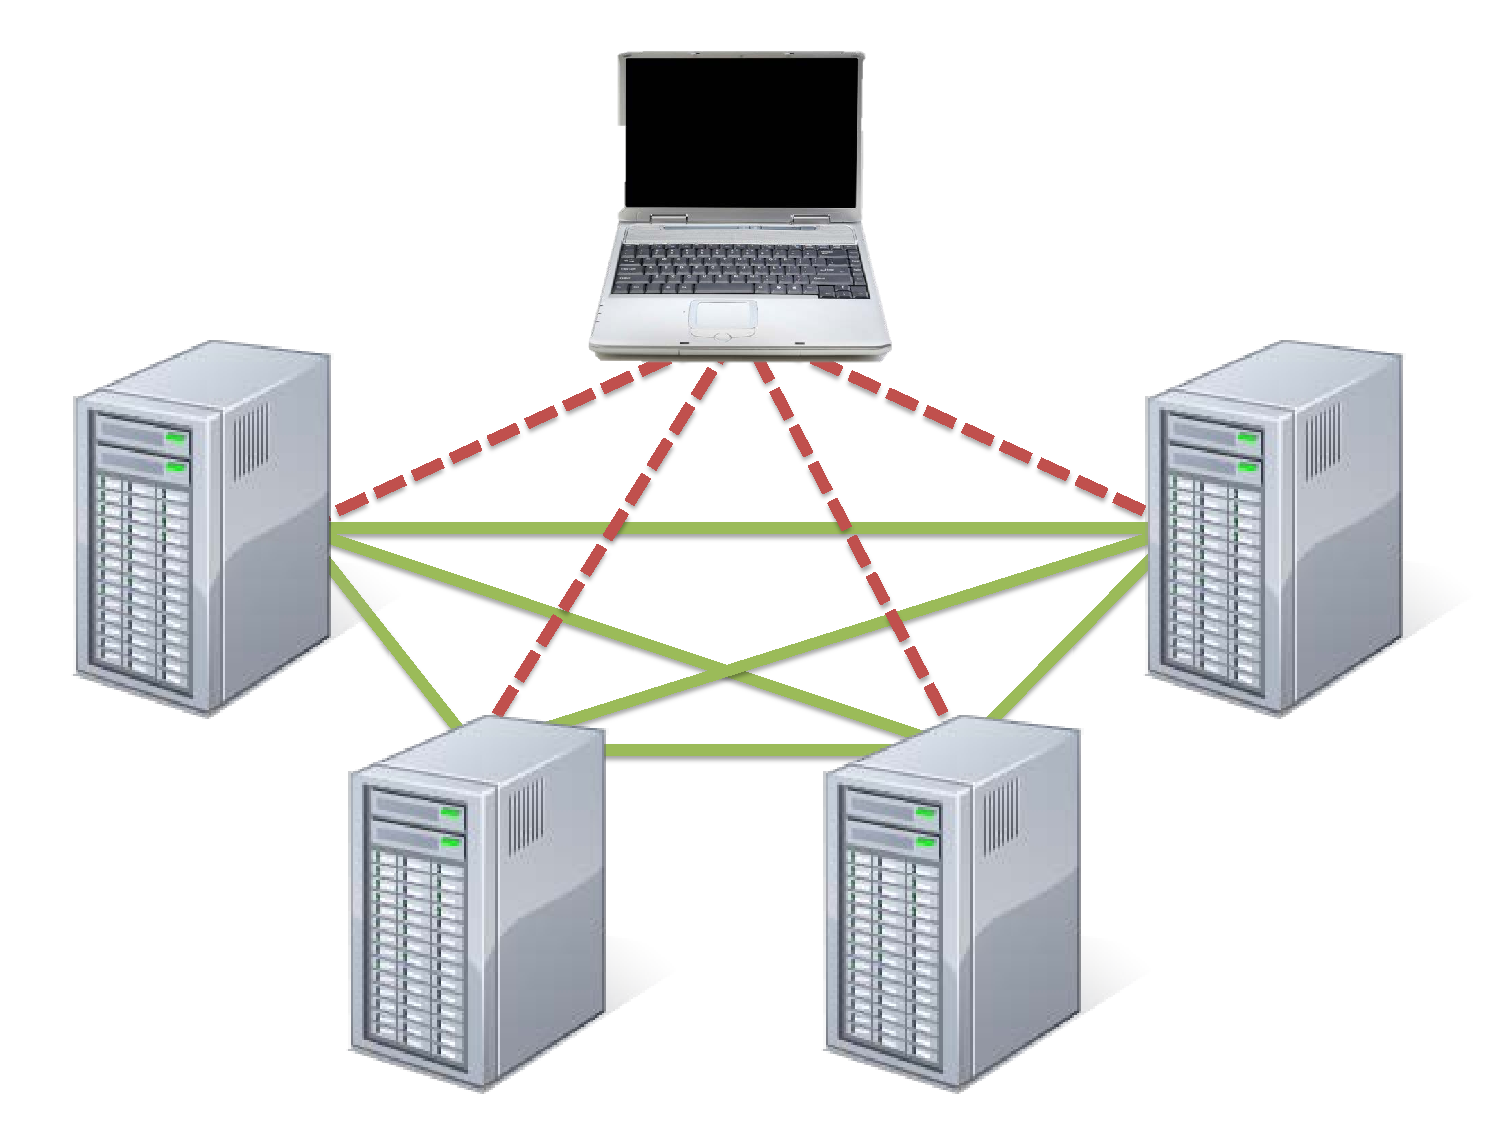
\includegraphics[width=100mm]{figures/netarch.pdf}
    \captionfonts
    \caption{Workers maintain connections with all other workers in the cluster. The renderer does the same.}
    \label{fig:netarch}
\end{figure}

\subsection{Fat Rays}
\label{fatrays}

The currency of computation and core message type in FlexRender is the
\emph{fat ray}. They are so named because they carry additional state
information along with their geometric definition of an origin and a direction.
Their counterparts, \emph{slim rays}, consist of only the geometric components.

Specifically, a fat ray contains the following data:

\begin{itemize}
    \item The \textbf{type of ray} this is. Described in Section \ref{process}.
    \item The \textbf{source pixel} that this ray contributes to.
    \item The \textbf{bounce count}, or number of times this ray has reflected
        off a surface (to prevent infinite loops).
    \item The \textbf{origin and direction} of the ray.
    \item The ray's \textbf{transmittance}, or the amount that it contributes
        to the source pixel.
    \item The \textbf{emission} from a light source carried along the ray (if
        any). Described in Section \ref{illumination}.
    \item The \textbf{target intersection point} of the ray, if any. Described
        in Section \ref{illumination}.
    \item The \textbf{traversal state} of the top-level BVH. Described in
        Section \ref{traversal}.
    \item The \textbf{hit record}, which contains the worker, mesh, and $t$
        value of the nearest intersection.
    \item The \textbf{current worker} this ray should be sent to over the
        network.
    \item The \textbf{number of workers touched} by the ray so far. Not
        necessary for rendering. Only used for analysis.
    \item A \textbf{next pointer} for locally queuing rays as described in
        Section \ref{queues}. Obviously not valid over the network.
\end{itemize}

In total, the size of a fat ray is 128 bytes.

\subsection{General Types}
\label{types}

The core graphics machinery in FlexRender is fairly straightforward. A scene consists
of a collection of \emph{meshes}, which are stored as indexed face sets of vertices
(positions with normals and texture coordinates) and faces.

Each mesh is a assigned a \emph{material}, which is responsible for drawing the
mesh. A material consists of a \emph{shader} and potentially a set of bindings
from \emph{textures} to names in the shader.

A \emph{shader} is a piece of code that is run to compute the lighting on a
surface at a particular point.

A \emph{texture} is a either a 2D array of pixels (for image textures) or
a snippet of code (for procedural textures) that defines the value of
something across a surface. They are most commonly used for providing colored
detail across the face of a triangle.

All of the code used in graphics computation is shared between both our baseline
implementation and FlexRender. This ensures fair comparisons when we analyze our
results in Section \ref{results}.

\subsection{Overview}
\label{overview}

In general, rendering with FlexRender proceeds in the following way:

\begin{enumerate}
    \item The renderer reads in the scene data and defines the maximum bounding
        extents of the entire scene. As data is read in, it is distributed to
        the workers using the Morton coding.
    \item Once the scene is distributed, workers build BVHs in parallel for
        their respective ``chunk" of the scene. They share their maximum bounding
        extents with the renderer.
    \item The renderer constructs a ``top-level" BVH from the worker bounds and
        shares this BVH with all the workers.
    \item Each worker creates its own image buffer. This is where any shading
        data will be written if it occurs on this worker.
    \item Each worker begins casting primary rays from the camera and tests for
        intersections (to find the nearest geometry that the ray hits).
        \begin{itemize}
            \item During intersection testing, rays may be forwarded over the
                network to another worker if they travel through the bounding
                extents of that worker.
            \item Once the nearest intersection is found illumination rays are
                created and sent to workers that have lights. These workers
                send light rays back towards the point of intersection to test
                for occlusion.
            \item If the light rays reach the intersection, the point is shaded
                because it is in direct view of the light.
        \end{itemize}
    \item Once all rays have been accounted for, workers send their image
        buffers back to the renderer, which composites them all together into
        a final image.
\end{enumerate}

In the next few sections, we'll examine each part of this process in greater
detail.

\section{Render Preparation}
\label{prep}

Render preparation consists of ensuring that all the workers agree on the
basic rendering parameters, distributing the scene assets to each worker, and
building the distributed bounding volume hierarchy. We discuss configuration
and distribution in Section \ref{sync} and parallel construction of the BVH in
Section \ref{parallelbvh}.

\subsection{Configuration and Asset Distribution}
\label{sync}

The configuration consists of basic information about how the scene is to be
rendered, such as the image dimensions, the workers participating in the render,
etc. In addition, the configuration specifies the minimum and maximum bounding
extents of the scene. This is used in the asset distribution step for driving
the Morton coding discretization along each axis.

Once the renderer has read in the configuration, it opens client connections
to each worker and sends the configuration data to them. Similarly, each worker
opens a client connection to every other worker. These renderer/worker and
worker/worker connections remain open for the duration of the render.

The renderer then divides up the 63-bit Morton code address space evenly by the
number of workers participating and assigns a region of it to each one.

Finally, the renderer begins reading in and parsing the scene data. As each mesh
is loaded, the renderer takes the following actions:

\begin{enumerate}
   \item Computes the centroid of the mesh by averaging its vertices.
   \item Computes the Morton code of the mesh centroid. This determines
      which worker the mesh will be sent to.
   \item Ensures that any asset dependencies (such as materials,
      shaders, and textures) for this mesh have been sent to the designated worker.
   \item Sends the mesh data to the designated worker.
   \item Deletes the mesh data from its own memory.
\end{enumerate}

Although the current implementation reads scene data in at the renderer
and distributes it over the network, there is no inherent reason why it needs to
do so. For example, if all the workers have access to the scene data over network
storage, the renderer could simply tell each worker the range of the Morton code
address space it is responsible for and let them load the scene data themselves,
carefully throwing out any geometry that is not within their Morton bounds.

\subsection{Parallel Construction of Spatial Acceleration Structures}
\label{parallelbvh}

To accelerate intersection testing against each mesh, each worker first
constructs a BVH for every mesh it has. These BVHs are tied directly to the mesh
they accelerate. While building each BVH, the worker stores a list of the bounding
extents of each mesh.

Next, each worker builds a root BVH for the entire worker, which uses the mesh
extents for its leaf nodes. When testing for intersections locally, a worker
first tests against this root BVH to determine candidate meshes, then traverses
each mesh's individual BVH to compute absolute intersections. After construction
of this root BVH, the root node's bounding extents will describe the spatial
extent of all geometry located on that worker.

Once construction of all the local BVHs is complete, each worker sends its
total bounding extents to the renderer. Once the renderer has the bounding
extents of each worker, it constructs a final ``top-level" BVH of the workers.
The renderer then distributes this top-level BVH to all the workers, so that
everyone participating has an identical copy of it. This is a very quick and
lightweight process, since it is only dependent on the number of workers
participating in the render.

This top-level BVH will be used to direct where we pass rays over the network
in Section \ref{traversal}.

\section{Ray Processing}
\label{process}

At their core, workers are essentially just multithreaded ray processors. Once
rendering begins, they continually pull rays out of the ray queue (discussed in
Section \ref{queues}), schedule them onto the thread pool, and process them
when the thread is run. This processing step consists of testing for intersection,
potentially forwarding the ray to another worker (Section \ref{traversal}),
or computing shading values if the ray terminates (Section \ref{shading}).

As mentioned in Section \ref{fatrays}, fat rays have an associated type. There
are three different types of rays in FlexRender:

\begin{itemize}
   \item \textbf{Intersection rays} are rays whose sole purpose is to identify
      a point in space at which we would like to compute shading.
   \item \textbf{Illumination rays} are essentially copies of intersection
      rays that have terminated. They are sent to workers who have emissive
      geometry (described in Section \ref{illumination}).
   \item \textbf{Light rays} are Monte Carlo samples that contribute direct
      illumination to a point that a worker is shading (described in Section
      \ref{illumination}).
\end{itemize}

\begin{figure}[h!]
    \centering
    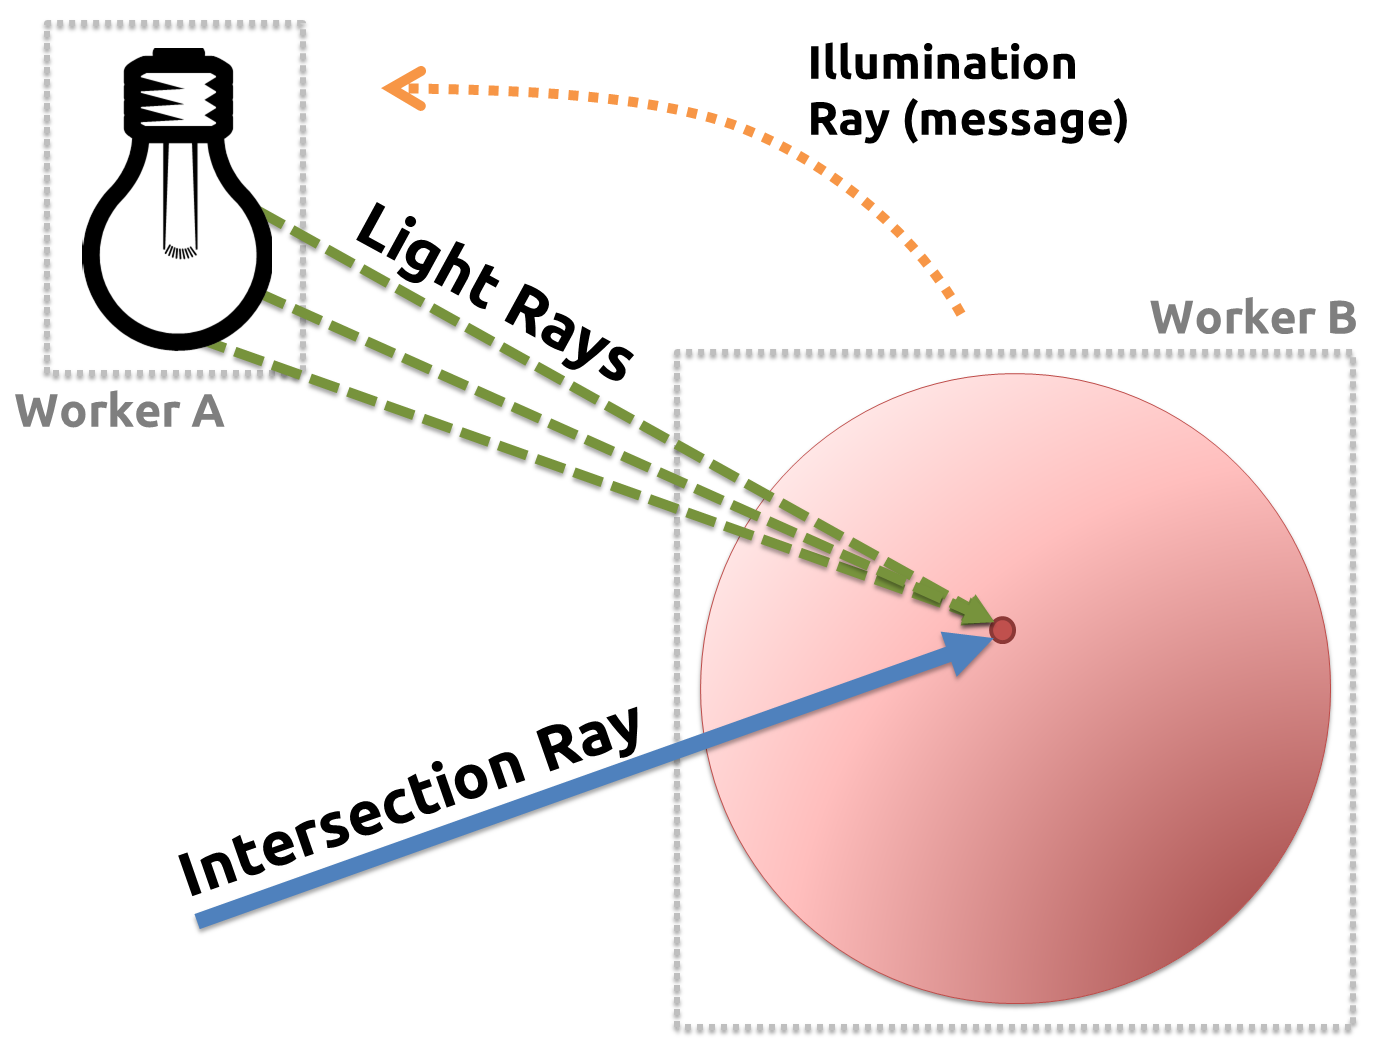
\includegraphics[width=120mm]{figures/raytypes.png}
    \captionfonts
    \caption{The three different ray types and their interactions.}
    \label{fig:raytypes}
\end{figure}

An important point to note about these rays is the sequence of their lifetimes.
Their purposes will become more clear in the following sections, but the order
is as follows:

\begin{enumerate}
   \item An intersection ray is cast into the scene.
   \item When that intersection ray terminates at a point in space, it dies and
      spawns illumination rays.
   \item When those illumination rays reach their destination, they die and
      spawn light rays.
   \item When those light rays terminate at a point in space, a shading value
      is computed.
\end{enumerate}

From this sequence of lifetimes, it should be apparent that a single intersection
ray can spawn many additional rays. It should also be apparent that light rays
are the most likely to die without generating more rays.

\subsection {Ray Queues}
\label{queues}

Each worker has a ray queue, with the typical push and pop operations for adding
and removing rays from the queue. This queue internally is implemented as three
separate queues, where rays are separated by type. It also contains information
about the scene camera, for generating new primary rays.

When a new ray arrives at a worker over the network, it is immediately pushed
into the queue. Internally, it is pushed into the queue matching its type
(intersection, illumination, or light).

When the worker pops a ray from the queue, we pull rays from the internal
queues in the following order:

\begin{enumerate}
   \item The \textbf{light queue}, since these are least likely to generate
      new rays.
   \item If the light queue is empty, we pop from the \textbf{illumination queue},
      since these will generate a limited number of new rays.
   \item If the illumination queue is empty, we pop from the
      \textbf{intersection queue}, since these can generate the most new rays.
   \item If all of the internal queues are empty, we use the camera to cast
      new primary rays into the scene (described in \ref{primaryrays}). This
      effectively generates new work.
\end{enumerate}

Organizing the processing order of rays as a priority queue based on ray type
is an essential step in minimizing the exponential explosion of work than can
occur if too many primary rays enter the system at a time. This helps reduce
memory usage required for queuing messages because new work is not generated
until the system is ready to handle it.

\subsection{Primary Ray Casting}
\label{primaryrays}

The workers in the cluster are each responsible for casting a portion of the
primary rays in the scene. The reasoning behind this is to give the cluster
the ability to regulate itself.

Consider the case where a worker has not received any work recently from other
workers in the cluster. For whatever reason (intersection tests, shading, etc.)
the other workers are too busy dealing with their own queues to send any work
in the direction of our lonely, rayless worker. By giving the worker control
over primary ray casting for a portion of the scene, we give workers the ability
to generate work when they have nothing to do.

However, to quote Uncle Ben, ``with great power comes great
responsibility". Consider the case where a worker contains mostly background
geometry. It will be receiving work from others infrequently because its size
in screen space is small, but yet it is in charge of casting primary rays for
a much larger slice of the image. In this case the worker may go on an
unfettered spree of primary ray casting, causing lots of grief for his fellow
workers since he is essentially generating work for others and little for
himself.

To prevent this ``runaway" case from overburdening the ray queues, we require
that workers report statistics about their progress to the renderer every so
often (10 times per second in the current implementation). If the renderer
notices that a worker is getting significantly further ahead of the others in
primary ray casting, we temporarily disable primary ray casting on that worker
until the others catch up.

Because the other workers will not generate primary rays as long as they still
have other rays in their queues to process, the priority queuing, shared
ray casting responsibilities, and temporary pausing of primary ray generation at
runaway workers provides a simple means of self-regulating the cluster that
works remarkably well and minimizing the memory overhead for message queuing.
We will examine the overhead in detail in Chapter \ref{results}.

\subsection{Distributed BVH Traversal}
\label{traversal}

To understand how distributed traversal of the top-level BVH works, consider
the following example traversal of this top-level tree with 5 workers (letters
A through E) participating in the render.

\begin{figure}[H]
    \centering
    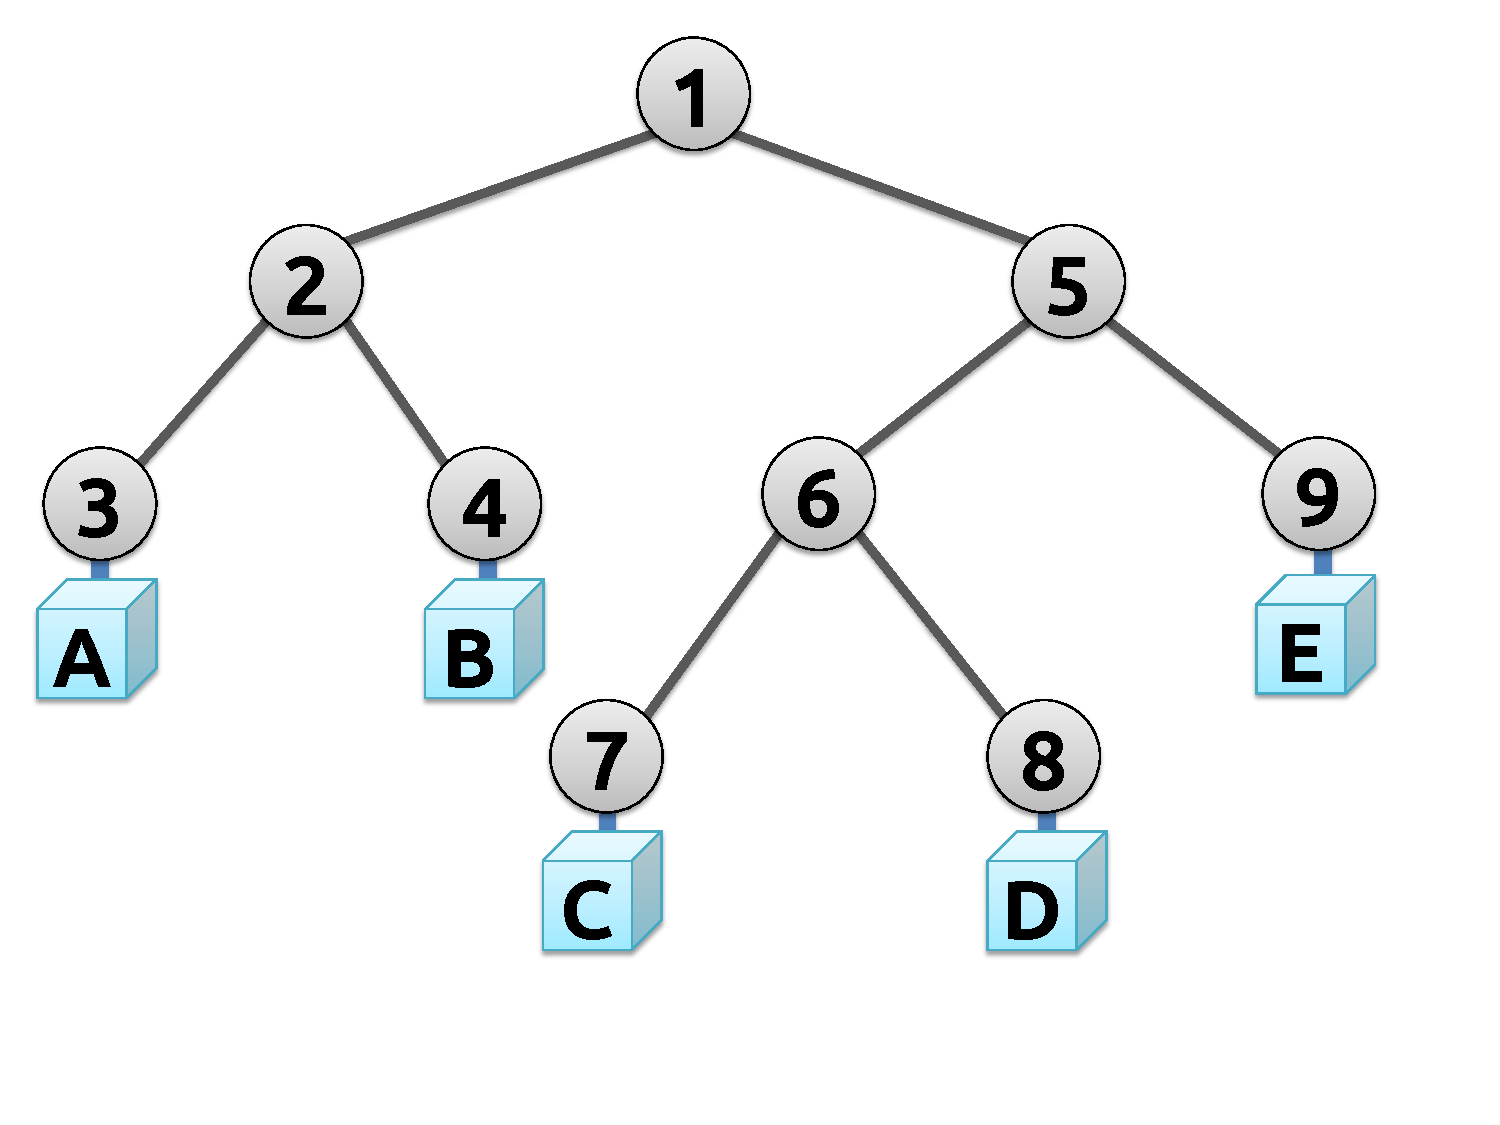
\includegraphics[width=100mm]{figures/traversal1.pdf}
    \captionfonts
    \caption{Example top-level BVH with 5 workers.}
    \label{fig:traversal1}
\end{figure}

The worker who generates the ray begins traversing the tree by checking the ray
against the bounds of the left-hand child. If the ray fails the test, we move
to check its sibling, right-hand child.

\begin{figure}[H]
    \centering
    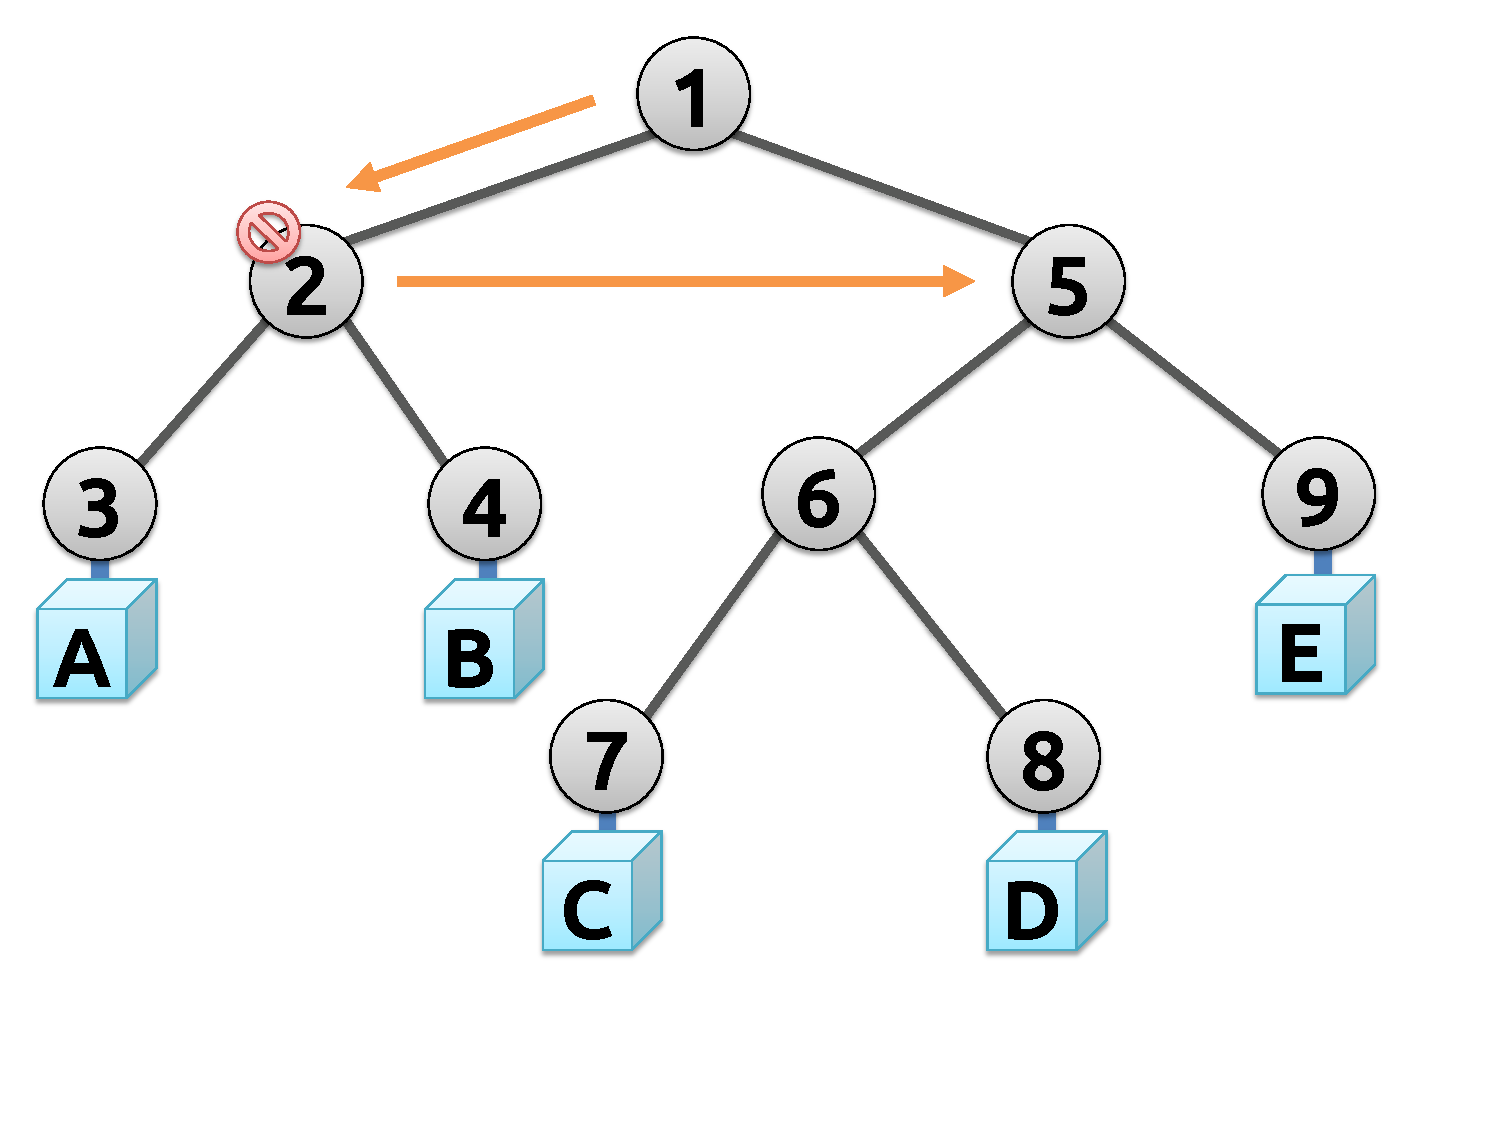
\includegraphics[width=100mm]{figures/traversal2.pdf}
    \captionfonts
    \caption{The ray fails its first test and moves to the sibling node.}
    \label{fig:traversal2}
\end{figure}

This test passes, so we continue down the tree to that node's left-hand child.
Let us assume this test also passes.

\begin{figure}[H]
    \centering
    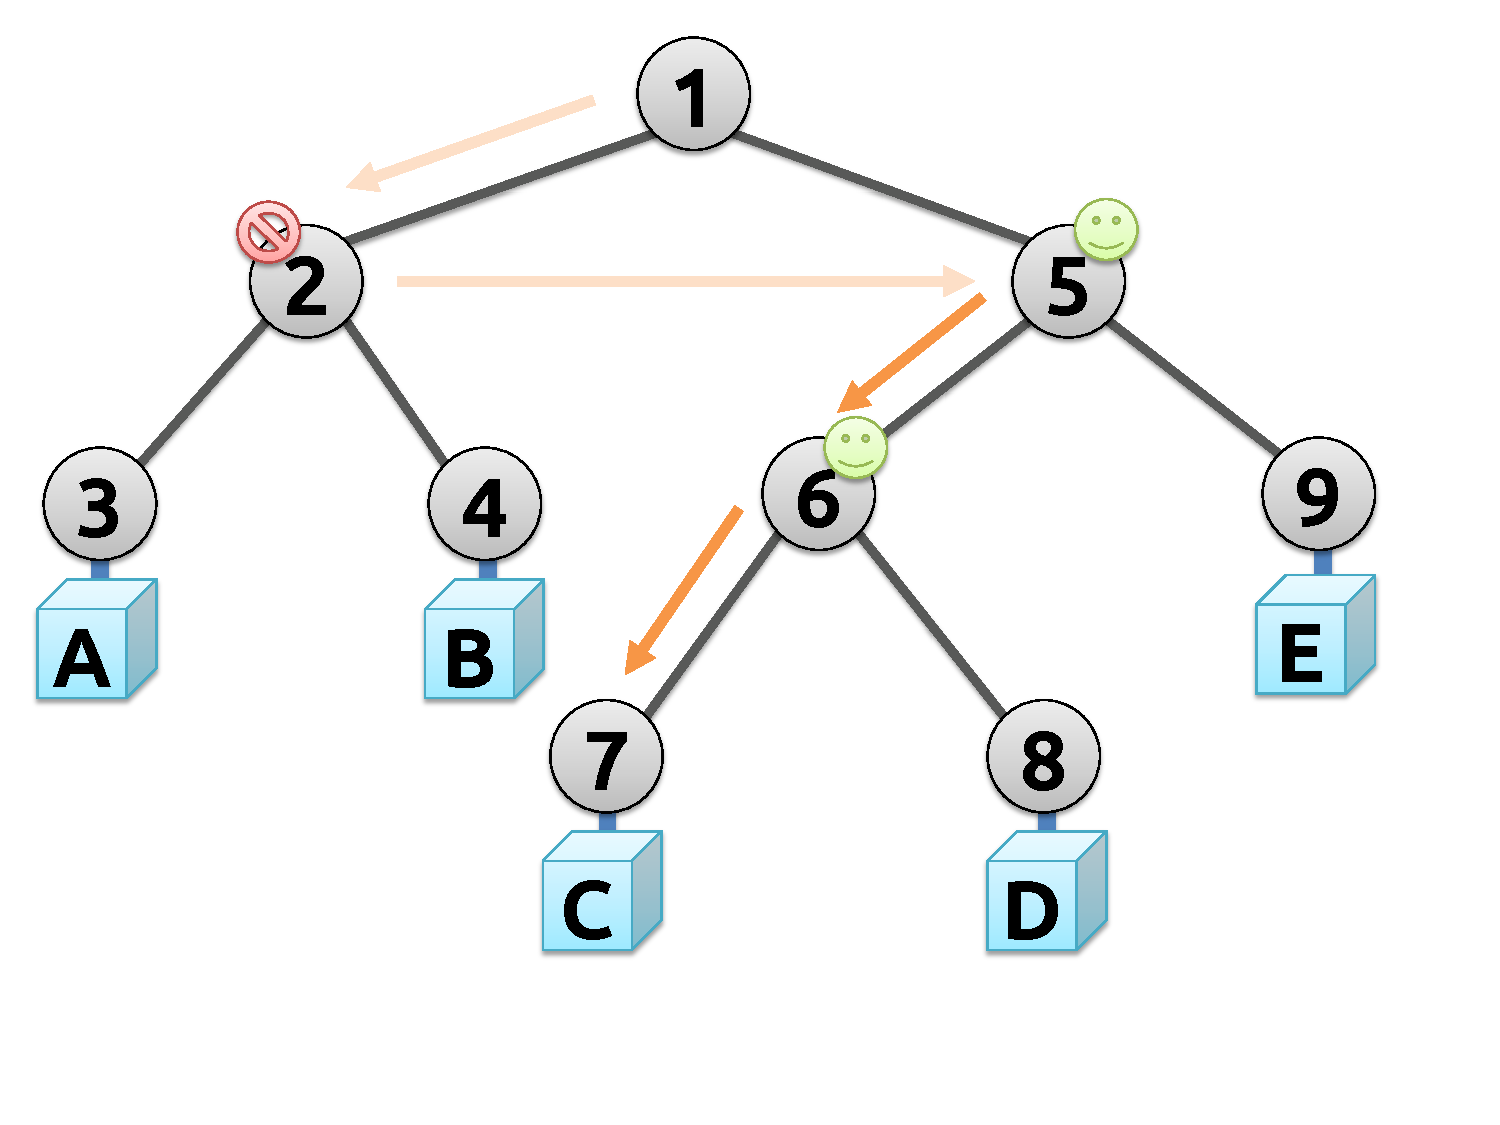
\includegraphics[width=100mm]{figures/traversal3.pdf}
    \captionfonts
    \caption{Traversal down the left-hand nodes continues as long as bounding tests pass.}
    \label{fig:traversal3}
\end{figure}

We test our first leaf node, and it passes. This indicates we must test the
geometry on the worker itself. This is where our primary modification to the
Hapala et al \cite{hapala:2011} algorithm occurs. Rather than continuing to
traverse the tree, we immediately jump out of the function the return the
traversal state. The traversal state consists of the index of the current
node, and the automaton defining where we came from (7 and \emph{from the parent}
respectively). We store this traversal state in the ray and pass it off to worker
C.

When worker C unpacks the ray and begins to process it, it notices that the
state of the traversal is not at the root of the tree, which means this is a
ray whose traversal was suspended. Because a suspended ray would never be sent
to a node for any other purpose than an intersection test, worker C immediately
tests for intersections against its geometry. For the purpose of this example,
let's say it hits nothing.

\begin{figure}[H]
    \centering
    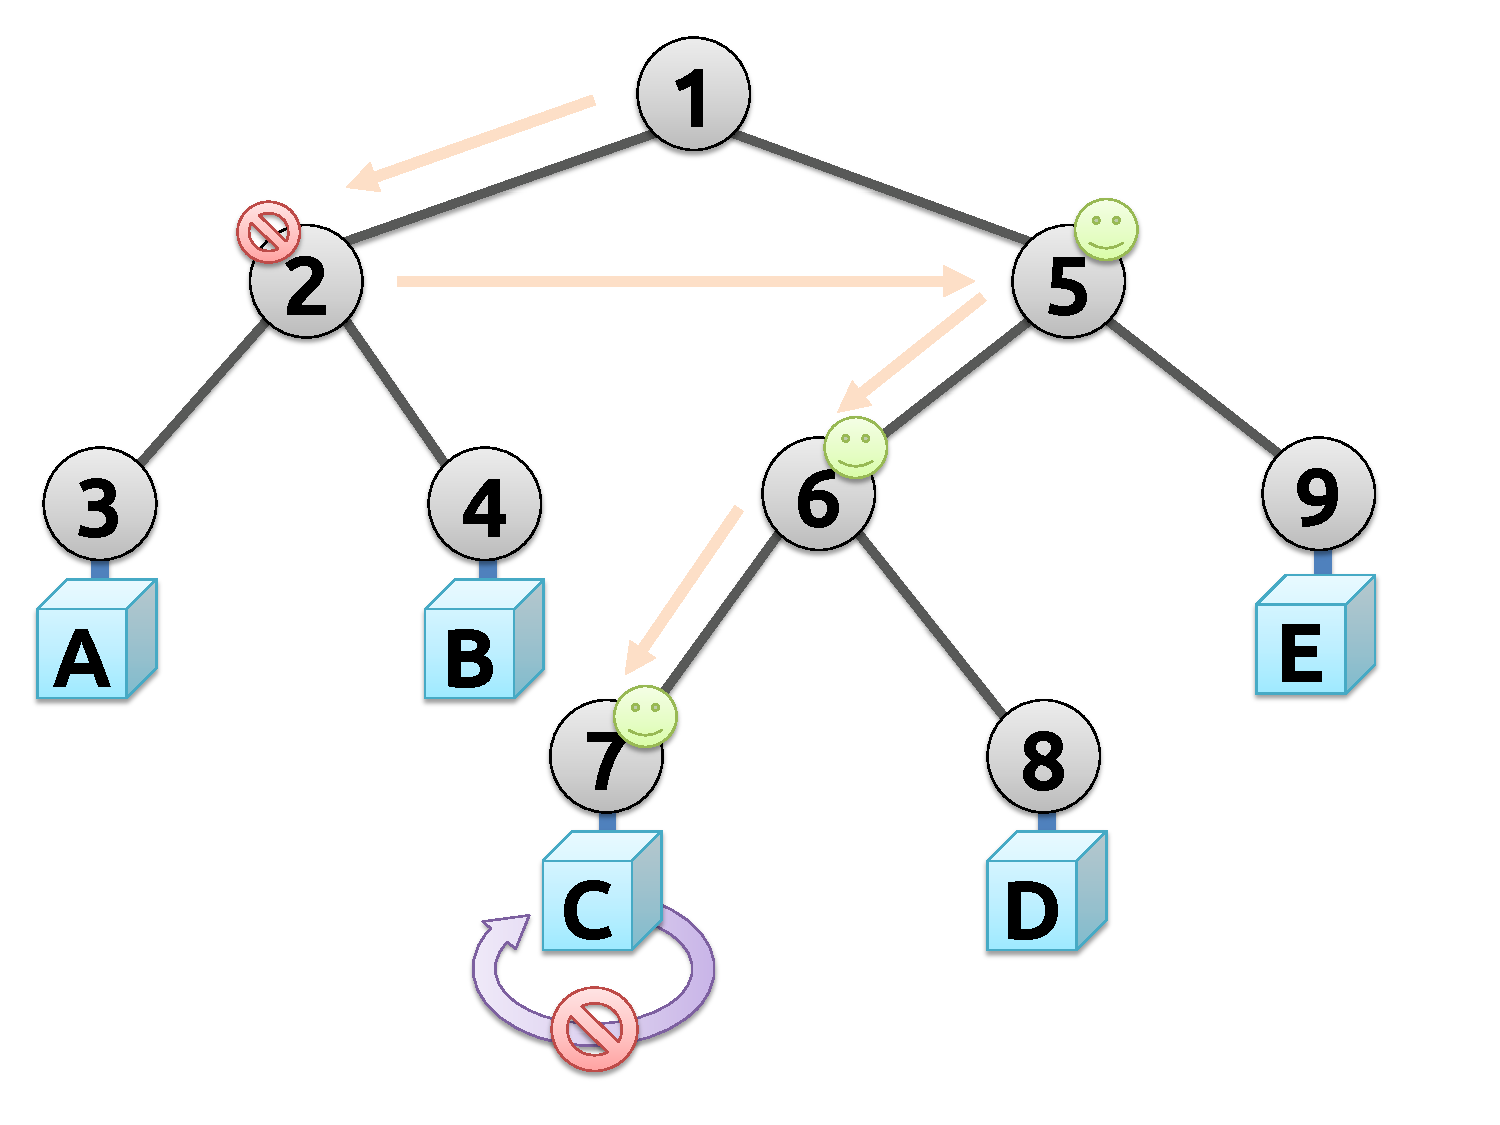
\includegraphics[width=100mm]{figures/traversal4.pdf}
    \captionfonts
    \caption{The ray is sent to worker C and tested against local geometry for intersections.}
    \label{fig:traversal4}
\end{figure}

The traversal state is then reinstated (node 7, \emph{from the parent}) and
worker C jumps immediately to where it left off, testing the bounds of C's
sibling, worker D. It hits the bounds, so again, we pack up the traversal
state (now node index 8 and \emph{from the sibling}) and ship off the ray to
worker D.

\begin{figure}[H]
    \centering
    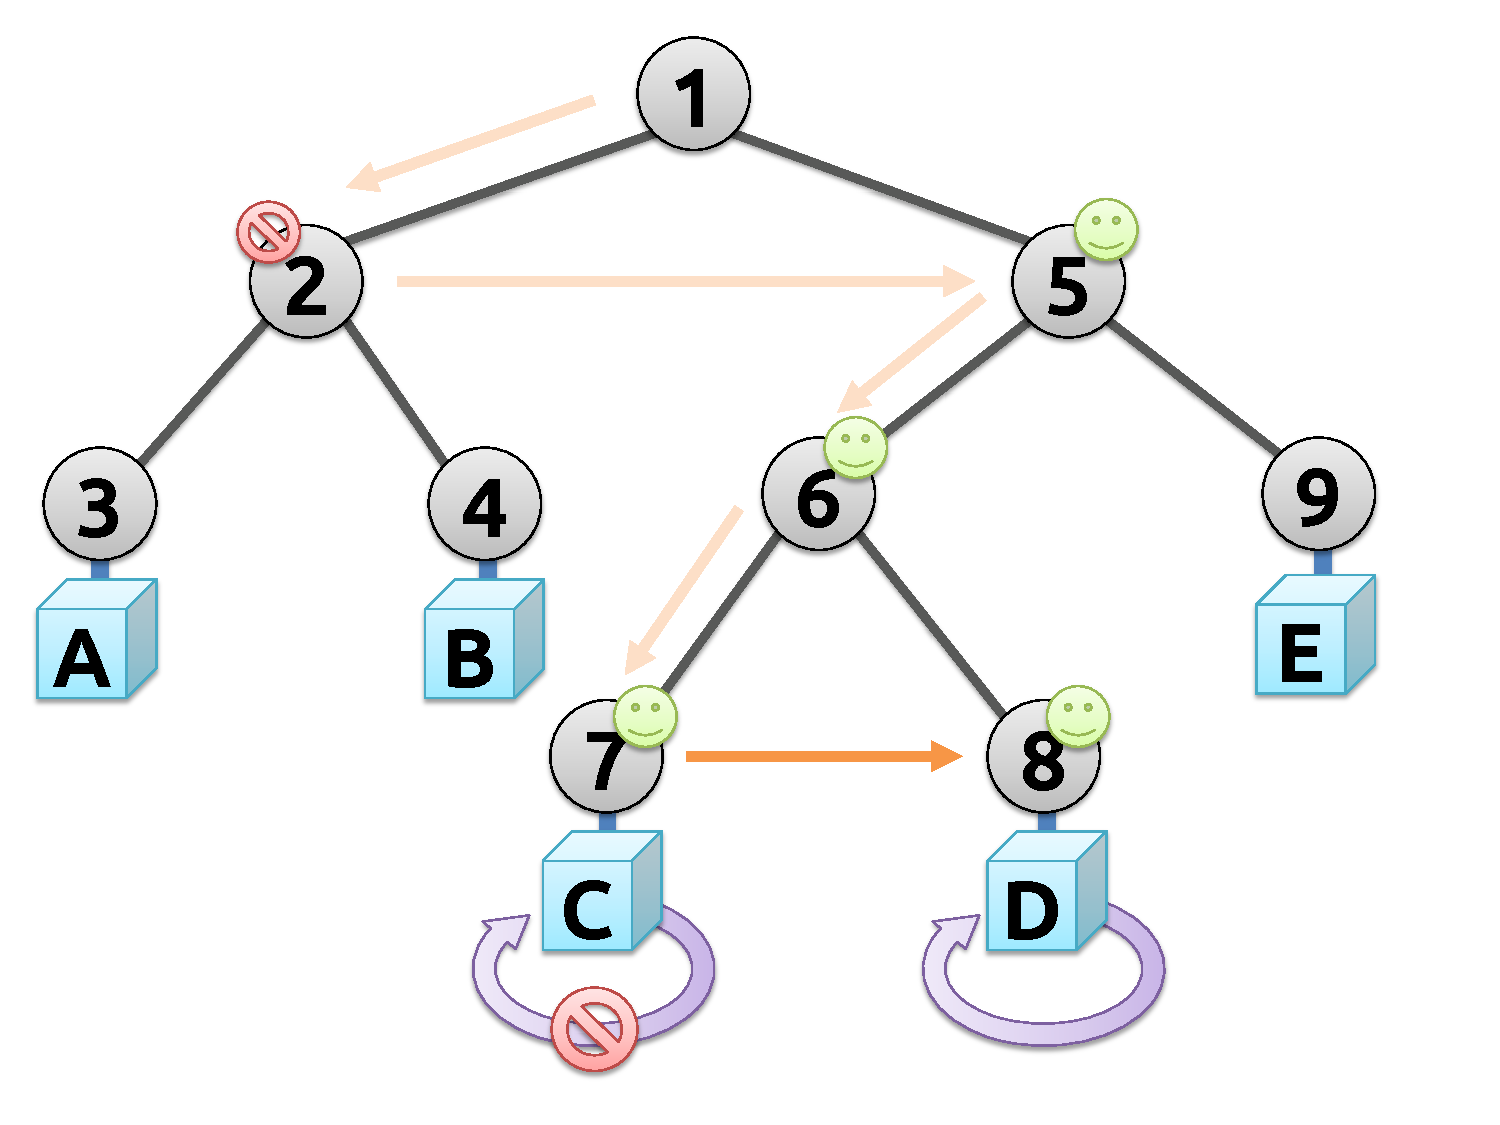
\includegraphics[width=100mm]{figures/traversal5.pdf}
    \captionfonts
    \caption{The ray is sent to worker D and again tested against local geometry for intersections.}
    \label{fig:traversal5}
\end{figure}

Worker D goes through the same process. Since the ray is suspended, it checks
its local geometry for intersections. Let's say it hits a mesh 42 at distance
of 10 units along the ray. This forms a hit record, which is stored inside the
ray (worker D, mesh 42, 10 units).

Again we reinstate the traversal state (node 8, \emph{from the sibling}) and
traverse back up to the parent (node 6). Since our state entering node 6 is
\emph{from the child}, we move next to node 9, another leaf node, and test
its bounds against the ray.

\begin{figure}[H]
    \centering
    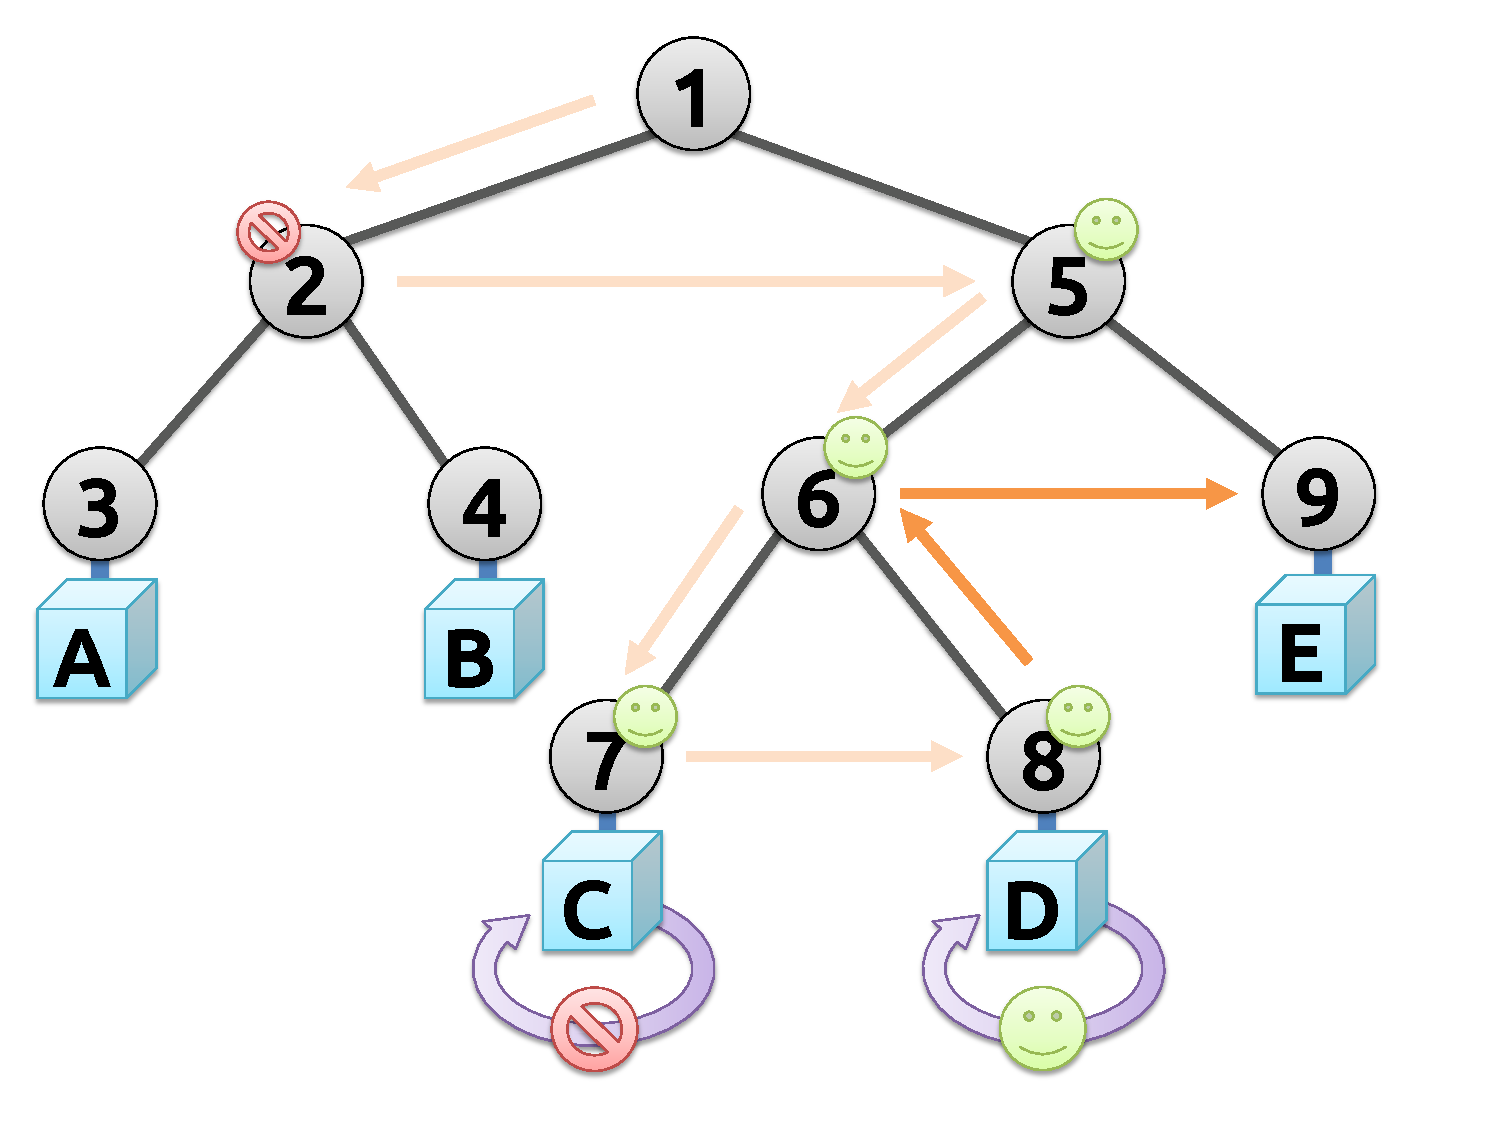
\includegraphics[width=100mm]{figures/traversal6.pdf}
    \captionfonts
    \caption{With successful hit record in hand, traversal continues back up the tree.}
    \label{fig:traversal6}
\end{figure}

Let's say this also passes. However, the ray intersects the bounds at a distance
of 20 units along the ray. The closest an intersection on worker E could
possibly occur is further away, so there is no point to sending the ray to
worker E. Thus, we don't send the ray to worker E and continue to traverse up
the tree until we reach the root again.

\begin{figure}[H]
    \centering
    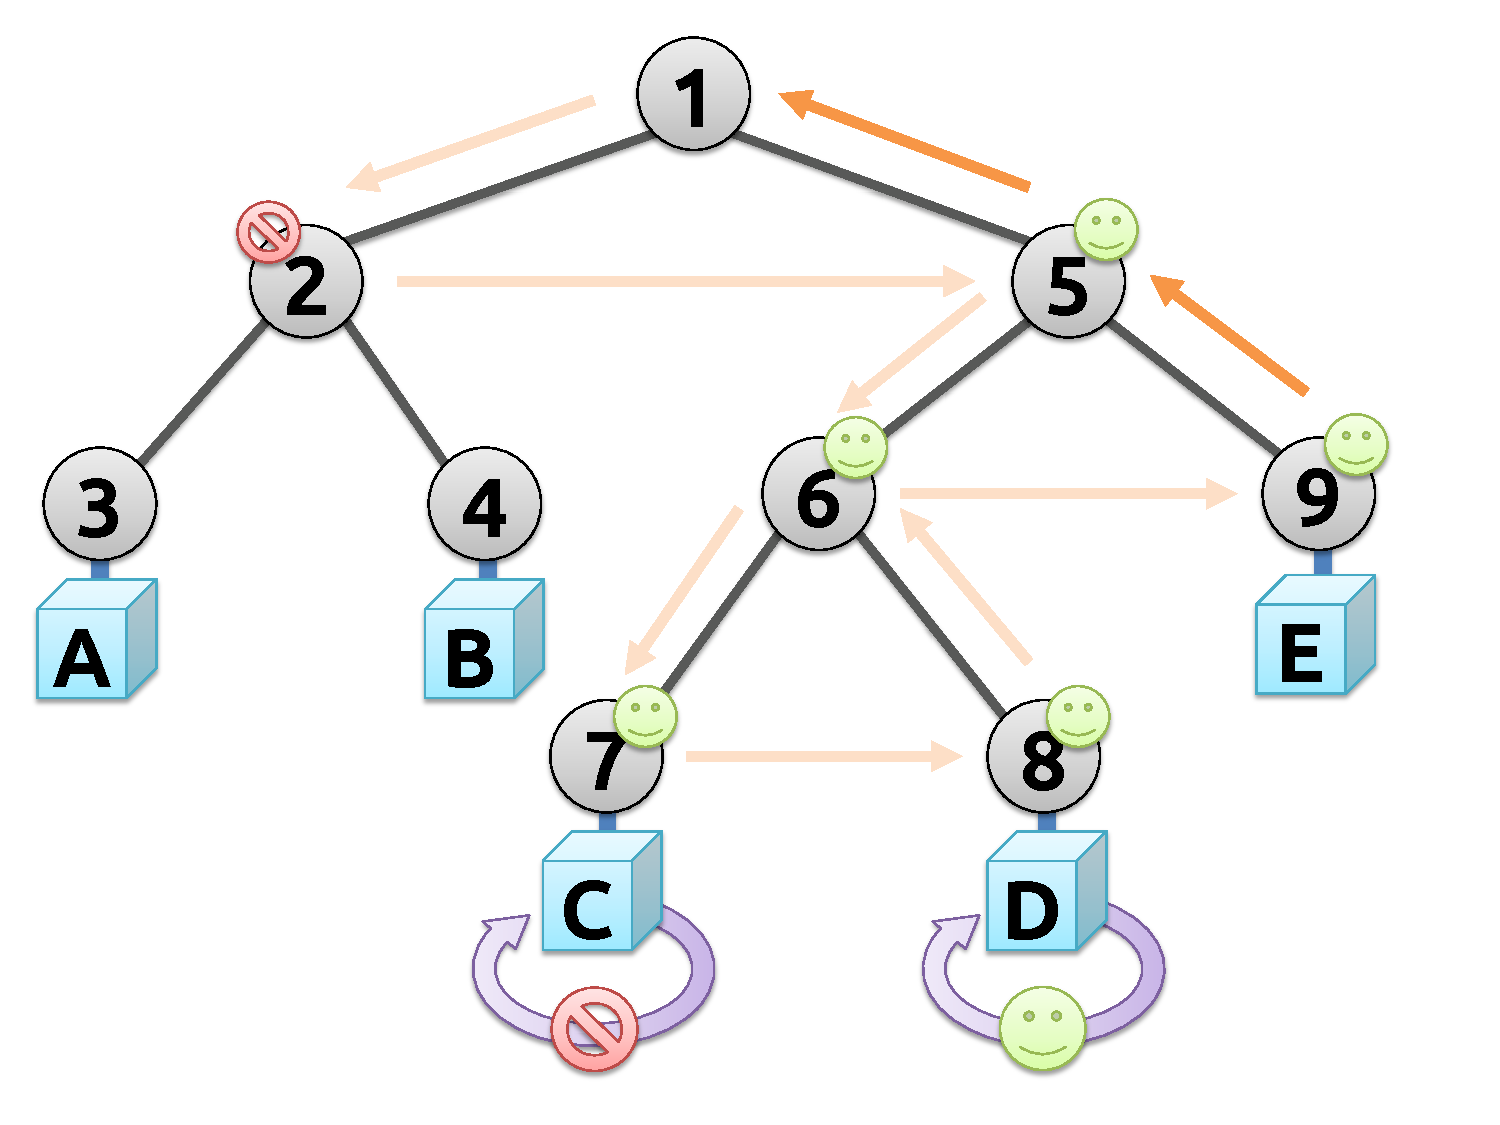
\includegraphics[width=100mm]{figures/traversal7.pdf}
    \captionfonts
    \caption{Worker E's bounding test passed, but was further away than the hit record. We arrive at the root and traversal is complete.}
    \label{fig:traversal7}
\end{figure}

Once we reach the root, we know the top-level traversal is complete. At this
point we only need to consult the ray's hit record to determine which mesh on
which worker yields the closest intersection.

In the best case, a ray is generated on, intersects only with, and is shaded on
a single worker. These rays never need to touch the network. In the worse case,
the ray potentially intersects with all nodes, so it must touch every node in
the tree before being sure of its intersection point.

In addition, there are two interesting corner cases to consider.

\begin{itemize}
    \item If the ray is generated on a node that it doesn't intersect until
        later in the traversal, it consumes one additional network hop at the
        very beginning of the traversal.
    \item If the ray completes its traversal on a worker different from that
        which had the closest intersection, it consumes one additional network hop
        at the end of the traversal to put the ray on the correct node for
        shading.
\end{itemize}

Thus, the worst case scenario actually touches $n + 2$ workers, where $n$ is the
number of workers in the cluster.

In Chapter \ref{futurework}, we discuss possible optimizations that may eliminate
both of these corner cases. Additionally in Chapter \ref{results}, we show that
in practice, the number of workers that each ray touches is less than or equal
to the predicted $O(log\;n)$ expansion of the binary tree for the majority
of rays in the scene.

\subsection{Illumination}
\label{illumination}

There is no special ``light" type in FlexRender, rather only meshes that are
emissive, which is a property set by the assigned material. Meshes that are
emissive are known to inject light into the scene through a special function in
their shader which is called to compute that emission. During scene loading,
the renderer maintains a list of all workers that have received at least one
emissive mesh. This list is synchronized with all workers right before
rendering begins.

Once a point has been identified for shading with intersection testing, we
need to determine the visibility of that point with respect to the light sources
in the scene. In a traditional ray tracer, you simply cast rays from the point
of intersection to samples on the surface of the light to determine visibility.
However in FlexRender, from the perspective of the worker doing the shading,
we have no idea where all the of the lights in the scene are, or more importantly,
if there is any geometry occluding the light and casting the intersection in
shadow.

To solve this problem, we simply trace the light rays in the opposite direction.
Rather than originating from the intersection point and heading in the
direction of the light, we originate the rays at the light and cast them in the
direction of the intersection point. To support area lights through Monte Carlo
integration, it is simply a matter of creating multiple light rays with origins
sampled across the surface of the light.

If the light ray arrives back at the original intersection point after being
traced through the cluster, we know that its path from the light was unoccluded.
This leverages the same efficient method for distributed ray tracing that we
already developed for testing intersections.

Specifically, casting light rays towards an intersection point consists of the
following operations:

\begin{enumerate}
    \item At the worker where an intersection was found, copy the ray data into
        an illumination ray with the target set to the point of intersection.
    \item Send this illumination ray to all workers known to have emissive meshes.
    \item When a worker receives an illumination ray, generate sample points
        across the surface of all emissive meshes. Set these sample points as
        the origins for new light rays.
    \item Set the directions of all the light rays such that they are pointed
        in the direction of the target (the original point of intersection).
    \item Push each light ray into the ray queue and let the cluster process
        them as usual.
\end{enumerate}

\subsection{Shading}
\label{shading}

When a light ray arrives at a worker, we simply check that its point of
intersection is within some epsilon of the target. If it is, we consider the
light sample visible, look up the material, shader, and textures for the mesh,
and run the shader. The shader is responsible for writing its computed values
into the worker's image buffer.

The implementation of shaders in FlexRender is through extensions to the Lua
\cite{lua} programming language, using the LuaJIT \cite{luajit} implementation
for speed. A shader may do any (or none) of the following:

\begin{enumerate}
    \item Sample textures based on the name bindings assigned in the material
        definition.
    \item Compute a light value based on some implementation of a mathematical
        shading model (such as the Phong model) and local information at the
        point being shaded (such as the interpolated surface normal and texture
        coordinates).
    \item Accumulate computed light values into the primary RGB buffers, or
        any auxiliary named buffer.
    \item Cast additional rays into the scene.
\end{enumerate}

\begin{lstlisting}[caption=Example of a simple Phong shader.,label=phongshader]
    function direct(view, normal, texcoord, light, intensity)
        local NdotL = dot(normal, light)
        if NdotL < 0 then NdotL = 0 end
    
        local R = reflect(-view, normal)
        local VdotR = dot(reflect, view)
        if VdotR < 0 then VdotR = 0 end
    
        local diffuse = 0.6 * vec3(1, 0, 0) * intensity * NdotL
        local specular = 0.2 * intensity * (VdotR ^ 8)
    
        accumulate3("R", "G", "B", diffuse + specular)
    end
    
    function indirect(view, normal, texcoord)
        local ambient = 0.2 * vec3(1, 0, 0)
        accumulate3("R", "G", "B", ambient)
    end
\end{lstlisting}

When new rays are cast into the scene from a shader, the results of that trace
are not immediately available. Instead, the trace pushes the new rays into the
queue for processing and the traversal and shading systems ensure that the
result of secondary and $n$-ary traced rays will be included in the final image.

In order for linearity and energy conservation to be respected, certain values
are inherited from the parent ray. In particular, the source pixel is inherited
(so the ray contributes to the correct pixel in the final image) and the
desired transmittance along the new ray is multiplied with the transmittance of
the parent ray (to ensure energy conservation is preserved).

Casting rays from the shader can be used to implement several common visual
effects:

\begin{itemize}
    \item \textbf{Alpha masking} can be achieved by casting a new ray in the
        same direction with the full transmittance of the parent ray.
    \item \textbf{Reflection} can be achieved by casting a new ray in the
        reflected direction with some fraction of the transmittance based on
        the reflectivity of the surface.
    \item \textbf{Refraction} can be achieved by casting a new ray in the
        refracted direction with some fraction of the transmittance based on
        the index of refraction and opacity of the surface.
    \item \textbf{Monte Carlo global illumination} can be achieved by casting
        rays in random directions by sampling the hemisphere above the surface,
        with fractional transmittances based on the number of samples.
\end{itemize}

\section{Render Completion}
\label{completion}

In a traditional recursive ray tracer, determining when the render is complete
is a simple task. Once the last primary ray pops its final stack frame
the render is over. In FlexRender, however, no one worker (or the renderer, for
that matter) knows where the ``last ray" is. To determine when a render is
complete, the workers report rendering statistics to the renderer at regular
intervals, which are used for deciding when the render is finished. This decision
metric is discussed in Section \ref{stats}.

Once the render is complete, the renderer requests the individual image buffers
from each worker and reassembles them into the final output image. This process
is discussed in Section \ref{synthesis}.

\subsection{Statistics and Monitoring}
\label{stats}

For monitoring the progress of the render, the workers report general statistics
about their activities to the renderer at regular intervals (in our current
implementation, 10 times per second). In particular, the following four
statistics are useful for determining if the render has finished:

\begin{description}
   \item[Primary Ray Casting Progress] The amount of the worker's primary rays
      that have been cast into the scene.
   \item[Rays Produced] The number of rays created at the worker during this
      measurement interval. This includes new intersection rays cast from the
      camera or a shader, illumination rays created by terminating intersection
      rays, or light rays created by processing illumination rays.
   \item[Rays Killed] The number of rays finalized at the worker during this
      measurement interval. This includes intersection rays that terminated or
      did not hit anything, illumination rays that were destroyed after spawning
      light rays, or light rays whose final shading value was computed.
   \item[Rays Queued] The number of rays currently in this worker's ray queue.
\end{description}

In particular, if any worker has not finished casting its primary rays, we
know for certain the render is not complete. Secondly, if we observe that no
rays are produced, killed, or queued at any workers for some number of
consecutive measurement intervals, it is reasonable to assume that the render
has concluded.

Our current implementation (which reports statistics 10 times per second)
waits until it sees 10 consecutive intervals of ``uninteresting" activity on
the workers before declaring the render complete. We find this achieves a nice
balance between wanting to end the render as soon as it is legitimately
finished and risking concluding it too early.

\subsection{Image Synthesis}
\label{synthesis}

Once the render has been deemed ``complete", the renderer requests the image
buffers from each worker. Because all rendering was computed by respecting
linearity, computing a pixel in the final output image is just a matter
of summing corresponding pixels in the worker buffers.

This can yield some interesting intermediate images. Each worker's buffer
represents the light in the final image that interacts in some way with the
geometry present on that worker.

For direct light, this shows up as shaded samples where geometry was present
and black areas where it was not. For other effects such as reflections and
global illumination, it appears that the worker had access to the whole scene's
geometry all along, but this is just an optical illusion. Since the rays
carry with them the source pixel they contribute to (and this value is inherited
as new rays are spawned from the primary ray), a worker can end up contributing
to any pixel in the image as long as the light interacted in some way with the
geometry it controlled.

\begin{figure}[h!]
    \centering
    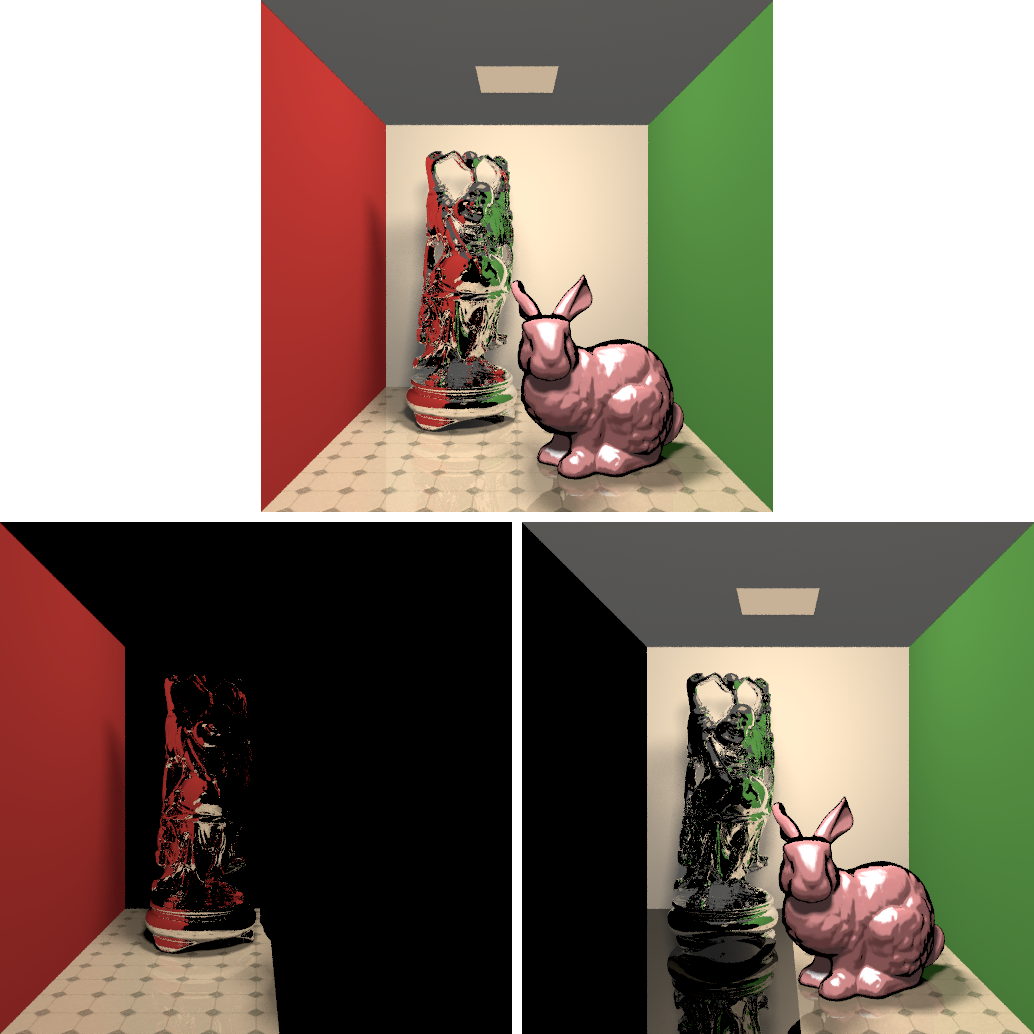
\includegraphics[width=140mm]{images/linearity.png}
    \captionfonts
    \caption{The left and right images show the geometry split between two workers. The composite image is in the center. Note how the Buddha reflects the left side geometry in the left image and the right side geometry in the right image. The actual Buddha mesh data was distributed to the worker on the left.}
    \label{fig:linearity}
\end{figure}

\chapter{Results}
\label{results}

\section{Experimental Setup}
\label{setup}

For testing, we used 2-16 Dell T3500 workstations with dual-core Intel Xeon
W3503 CPUs clocked at 2.4 GHz. Each workstation had 4 GB of system RAM, a 4 GB
swap partition, and was running CentOS 6.

On the software side, FlexRender consists of around 14,000 lines of code. Of
that, 80\% is C++ (with fairly extensive use of C++11), 17\% is Lua (scene and
shader support libraries), and 3\% is Bash script used for building library
dependencies.

We leverage several popular open source libraries:

\begin{itemize}
    \item \textbf{LuaJIT}, for a fast implementation of of the Lua programming language.
    \item \textbf{libuv}, the C library behind Node.js, for asynchronous networking and thread pools.
    \item \textbf{MsgPack}, for C++ class serialization.
    \item \textbf{GLM}, a C++ implementation of the GLSL math specification.
    \item \textbf{OpenEXR}, for writing full 32-bit float HDR images.
\end{itemize}

We also made use of the \textbf{pfstools} and \textbf{pdiff} software packages
for tone mapping our output images and computing perceptual diffs respectively.

\section{Toy Store}
\label{toystore}

Our test scene, ``Toy Store", has a geometric complexity of nearly 42 million
triangles. It consists of 1.09 GB of mesh data and 5 GB of BVH data once the
acceleration structures are built.

The room geometry is relatively simple, but the toys on the shelves are unique
(non-instanced) copies of the Stanford bunny, Buddha, and dragon models that
have been remeshed from their highest quality reconstructions down to 14,249
faces, 49,968 faces, and 34,972 faces respectively. There are 30 toys per
shelf and 42 shelves in the scene for a total of nearly 1,300 models. Approximately
one quarter of the models are rendered with a mirror shader. The others have
a standard Phong shader.

The image was rendered at a resolution of 1024x768 with no subpixel antialiasing,
10 Monte Carlo samples per light (32 lights in the scene), and a recursion
depth limit of 3 bounces.

\begin{figure}[h!]
    \centering
    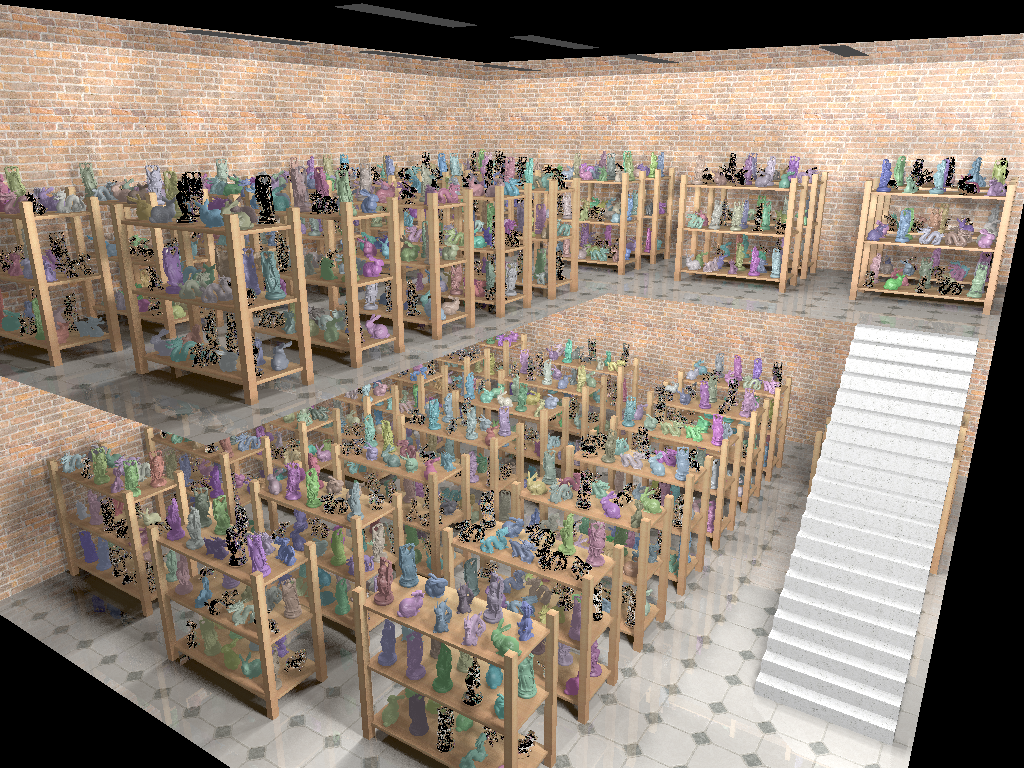
\includegraphics[width=140mm]{images/toystore.png}
    \captionfonts
    \caption{The ``Toy Store" scene used for benchmarking FlexRender.}
    \label{fig:toystore}
\end{figure}

\section{Render Time}
\label{rendertime}

For discussing render time speedups, we'll consider the specific case of 8
workers in the traditional configuration vs. 8 workers in the FlexRender
configuration. We'll cover other cluster sizes in less depth in Section
\ref{clustersize}.

\subsection{Traditional Method}
\label{toystoretraditional}

The traditional method works by chopping up the image into several vertical
slices, with a different machine responsible for each slice. The slices are
then reassembled to form the final output image.

\begin{figure}[h!]
    \centering
    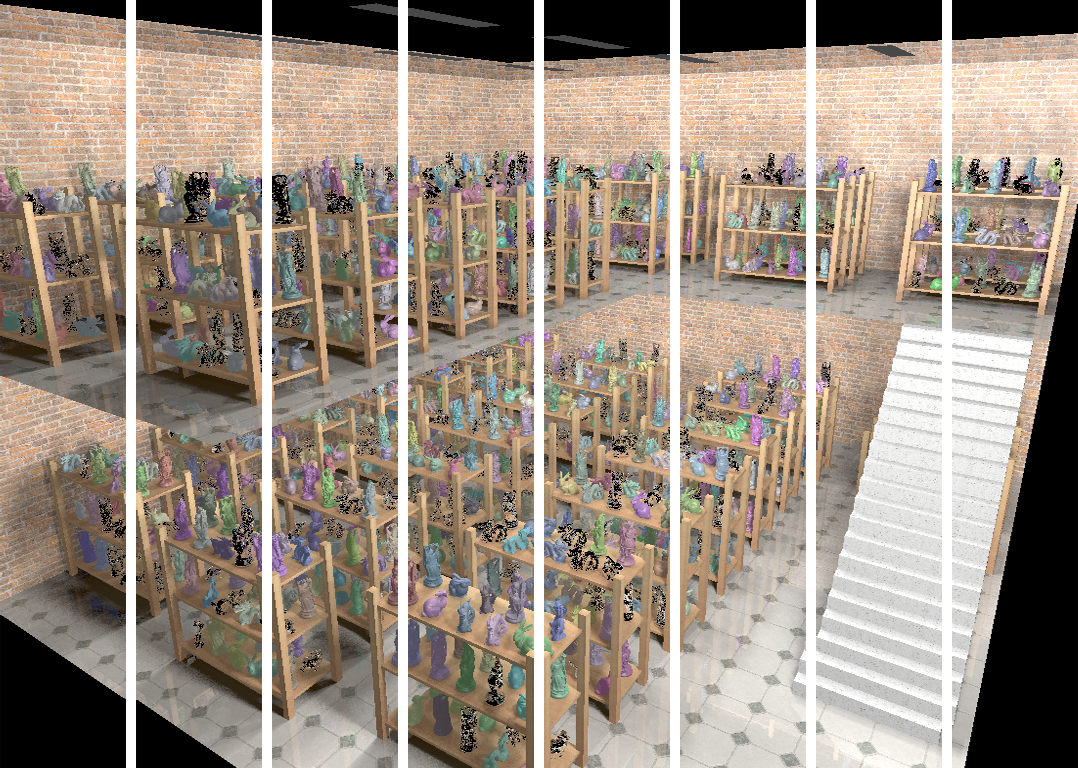
\includegraphics[width=120mm]{images/toystore-sliced.png}
    \captionfonts
    \caption{Slices of the Toy Store scene rendered with 8 machines in the traditional configuration.}
    \label{fig:toystoresliced}
\end{figure}

We report time for each machine to complete each phase of rendering (loading
the scene, building the BVH, and rendering its slice of the image) in Table
\ref{tb:traditionaltimes}. In particular, the total length of the render would
take 10,061 seconds (the slowest time), because the last slice is needed before
the final image can be reassembled.

\begin{table}
\begin{center}
\begin{tabular}{|l||c|c|c|c|c|c|c|c|}
    \hline
    & 1 & 2 & 3 & 4 & 5 & 6 & 7 & 8 \\
    \hline
    \hline
    Loading & 288 & 290 & 290 & 289 & 295 & 290 & 287 & 294 \\
    \hline
    Building BVH & 169 & 172 & 167 & 261 & 174 & 192 & 165 & 171 \\
    \hline
    Rendering & 533 & 1119 & 1491 & 9511 & 1792 & 677 & 1109 & 303 \\
    \hline
    \hline
    Total & 990 & 1581 & 1948 & 10061 & 2261 & 1159 & 1561 & 768 \\
    \hline
\end{tabular}
\caption{Time (in seconds) for individual workers to complete each phase using the traditional method.}
\label{tb:traditionaltimes}
\end{center}
\end{table}

\subsection{FlexRender}
\label{toystoreflexrender}

For comparison purposes, we report average times for the traditional workers
compared to FlexRender for each of the 3 rendering phases in Table
\ref{flexrendertimes}. We also show FlexRender's speedup over the average case.

We also report the total render time (all three phases combined), using this
time the slowest traditional worker. This is a fair comparison because even if
all of the other traditional workers finish quickly, the render is not complete
until the last worker finishes.

Lastly, we also report the times and speedup excluding the loading and syncing
phase. The reasoning behind this is that while FlexRender currently reads in
scene assets at the renderer and distributes them across the network, there is
no inherent reason why it needs to load the scene this way. Specifically,
if each worker had access to a shared network storage volume with the scene
assets on it, The renderer could simply issue commands to each worker
instructing it to load a particular asset from the network storage.

\begin{table}
\begin{center}
\begin{tabular}{|l||c|c|c|}
    \hline
    & Traditional & FlexRender & Speedup \\
    \hline
    \hline
    Loading & 290.4 (avg) & 326 & 0.89x \\
    \hline
    Building BVH & 183.6 (avg) & 20 & 9.18x \\
    \hline
    Rendering & 2066.9 (avg) & 1186 & 1.74x \\
    \hline
    \hline
    \textbf{Total} & \textbf{10061 (slowest)} & \textbf{1532} & \textbf{6.57x} \\
    \hline
    \textbf{Total (w/o loading)} & \textbf{9800 (slowest)} & \textbf{1206} & \textbf{8.13x} \\
    \hline
\end{tabular}
\caption{Time (in seconds) for each phase of rendering with FlexRender and the traditional configuration.}
\label{tb:flexrendertimes}
\end{center}
\end{table}

\begin{figure}[h!]
    \centering
    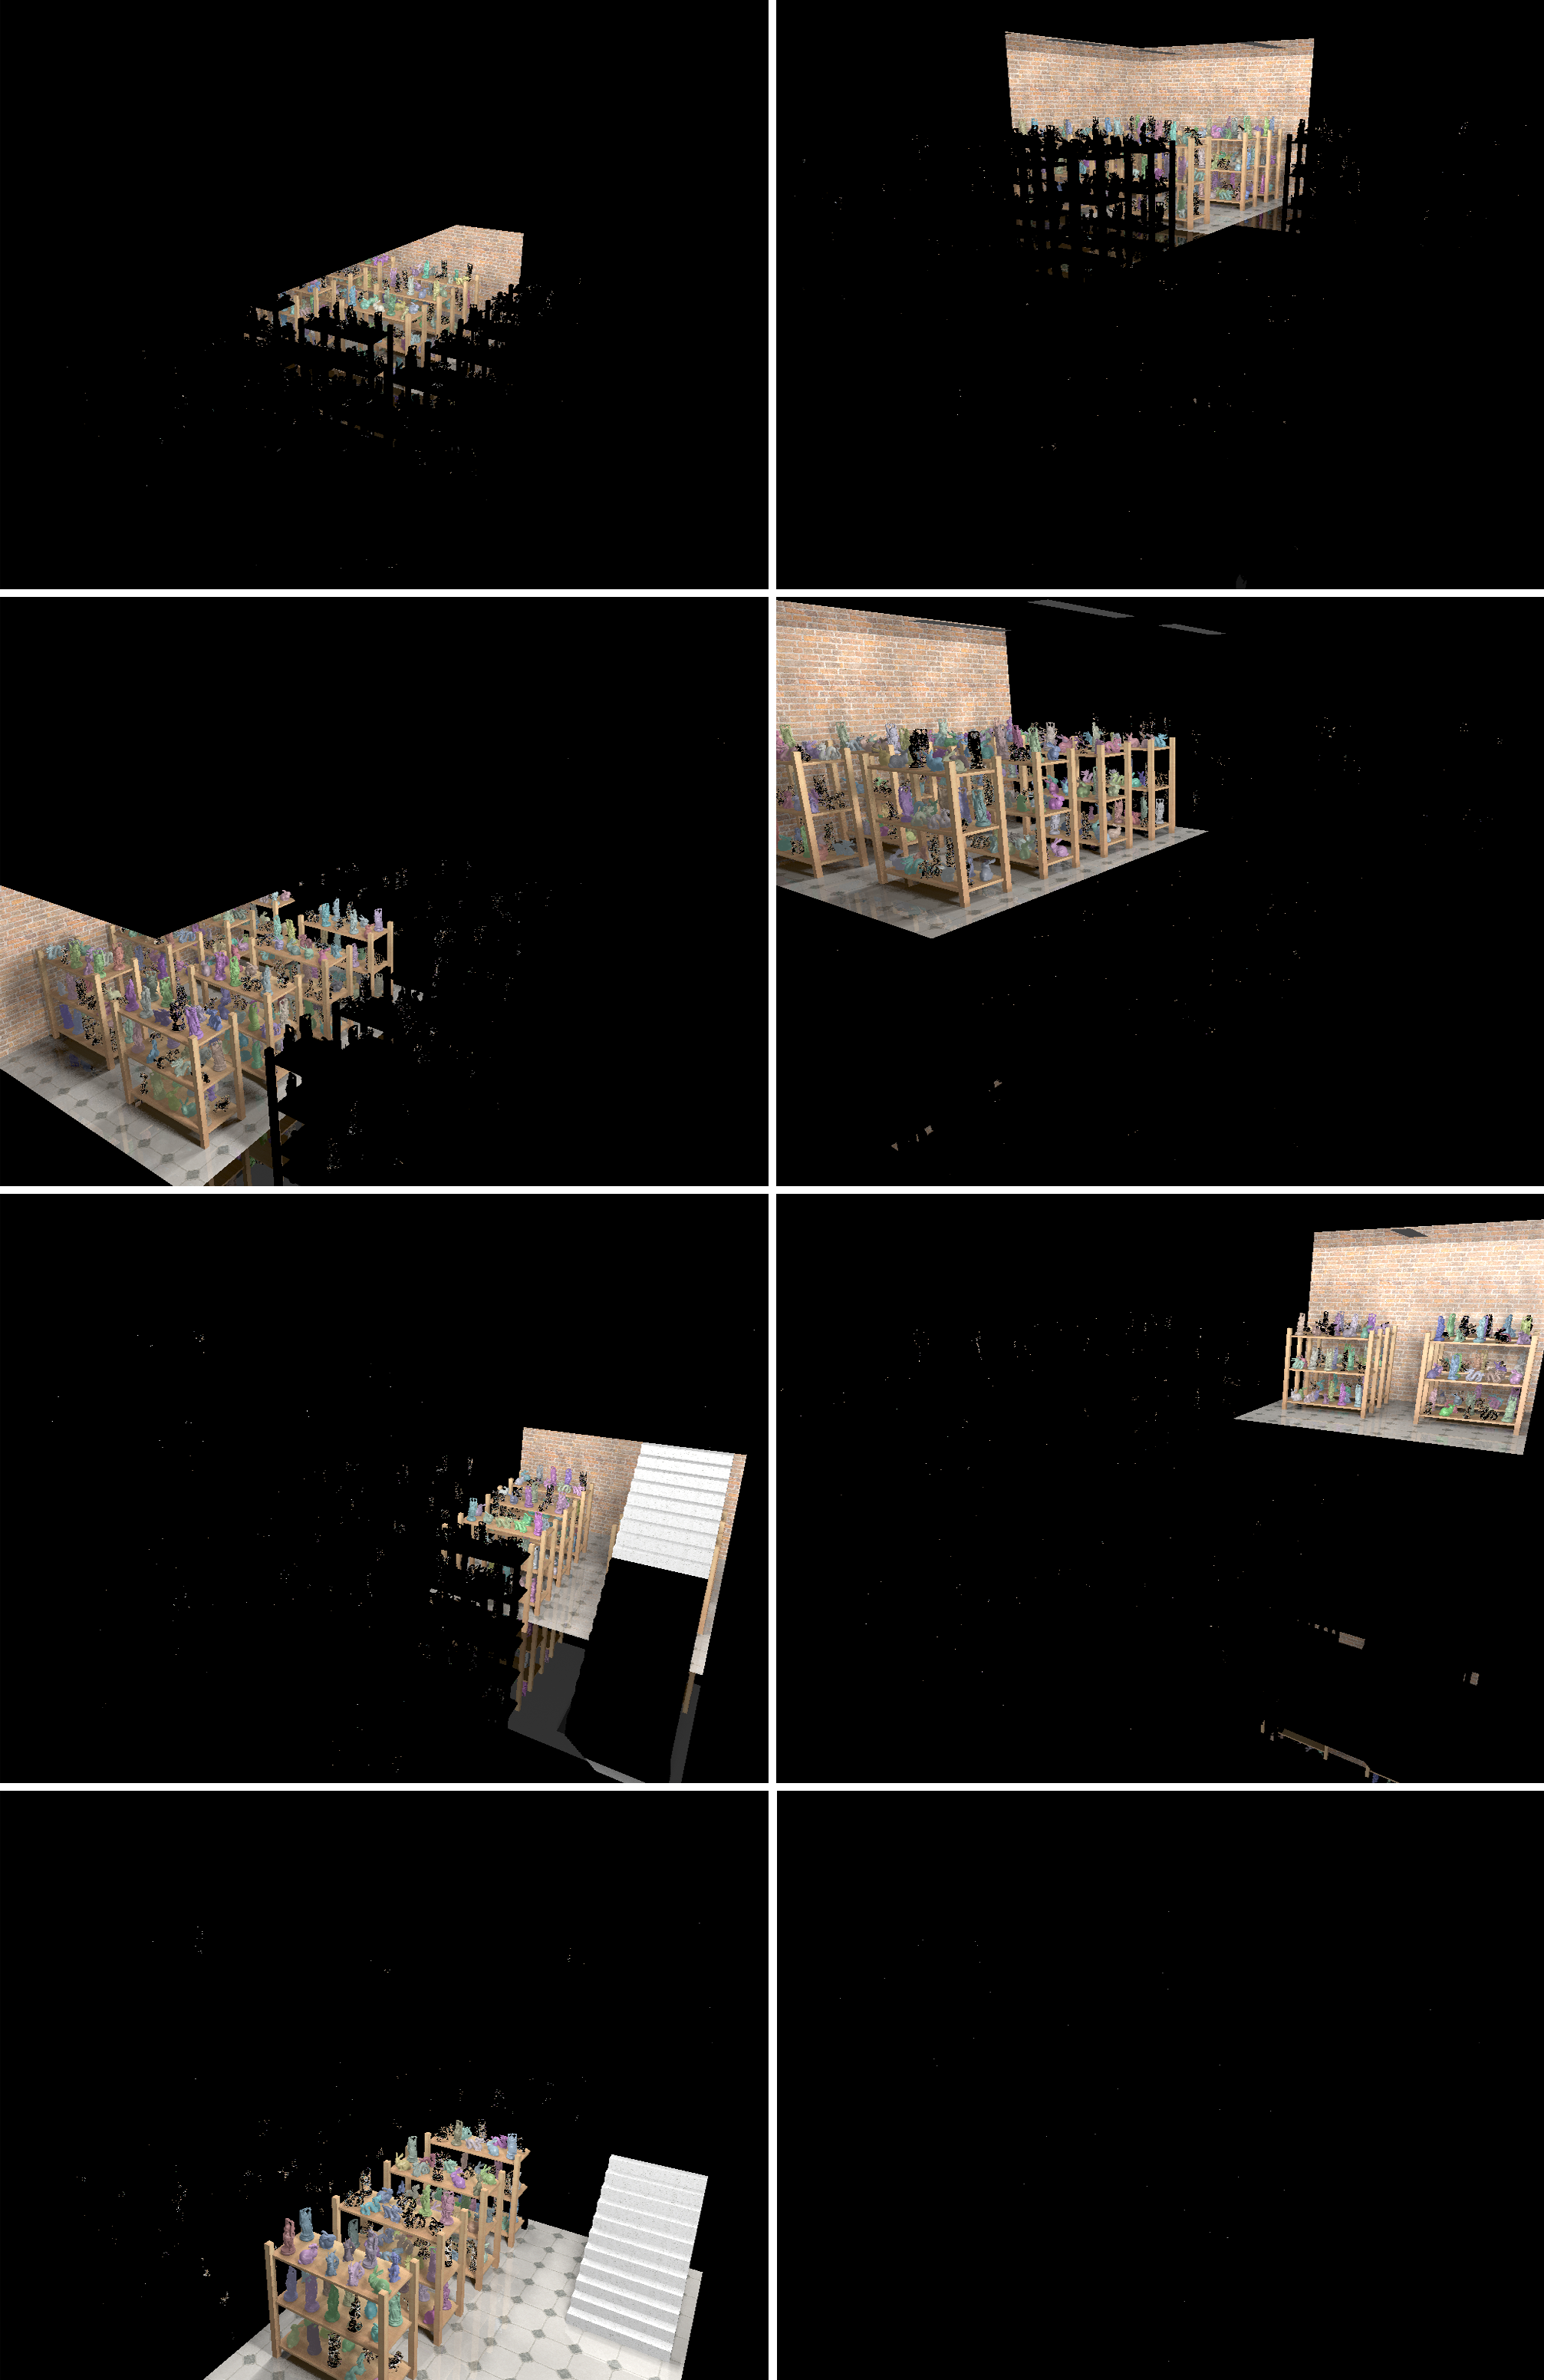
\includegraphics[width=120mm]{images/toystoredistribution.png}
    \captionfonts
    \caption{The individual worker image buffers that are combined to form the final image.}
    \label{fig:toystoredist}
\end{figure}

\section{Geometry Distribution}
\label{geomdist}

To ensure the entire scene stays in core, FlexRender must distribute the
geometry across the available RAM in the cluster effectively. With the exception
of one worker, the Morton coding and Z-order curve did a decent job of
partitioning the scene data evenly.

\begin{figure}[h!]
    \centering
    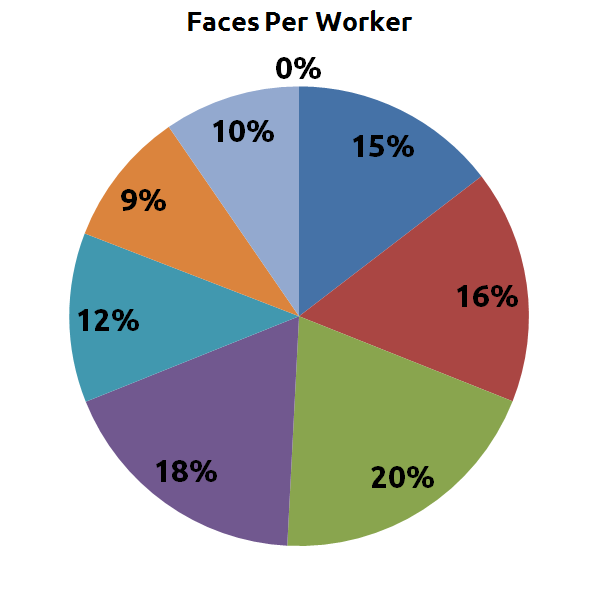
\includegraphics[width=80mm]{figures/facesperworker.png}
    \captionfonts
    \caption{Percentage of total geometry that was distributed to each worker.}
    \label{fig:geomdist}
\end{figure}

The one worker which did not contain very much geometry was in the top corner
of the Toy Store closest to the camera. This octant of the scene only contained
a fill light facing the rest of the geometry.

\textbf{TODO: geometry distribution table}

\section{Network Hops}
\label{nethops}

The intent of the top-level BVH is to reduce network cost by only sending
a ray across the network when we know it ventures into that worker's region
of space. Since a BVH is a $O(log\;n)$ data structure, we expect that with 8
workers the average ray would be handled by 3 workers during its lifetime.

\textbf{TODO: workers touched table}

Our results show that 63.2\% of rays are handled by 3 workers or less, and
nearly 16\% of them never even go out over the network (they are generated on,
intersect with, and are shaded on a single worker). We also see that 36.8\% of
rays must touch more than the expected 3 workers.

However, if we include the edge cases mentioned in \ref{traversal}, we see that
82\% of rays are at or below $O((log\;n) + 1)$ and 90.9\% of rays are at or
below $O((log\;n) + 2)$. In Section \ref{networkhop} we discuss some potential
methods for reducing or removing these extra network hops.

\section{Ray Queue Sizes}
\label{queuesizes}

Keeping the ray queue size small is critical to the long term health of the
render. If rays begin piling up faster than the cluster can process them,
eventually the cluster will begin swapping when accessing rays, which violates
our fundamental performance goal to stay off of disk.

Because of this, we benchmarked the ray queue sizes on each worker over time
when rendering Toy Store on a cluster of 16 workers. Figure \ref{fig:queuesize}
shows this with each renderer displayed as a different color. Table \ref{tb:rayqueues}
breaks down the average queue size, as well as the maximum size over the course
of the entire render and the storage requirements of the maximum size, both in
terms of raw storage space and a fraction of the system RAM.

As Table \ref{tb:rayqueues} shows, most workers sit comfortably below 1\% of
their RAM being used for queued rays, while the busiest worker used just over
1\%. This demonstrates that our regulation mechanisms and work throttling is
working well to keep the cluster from generating more work than it can handle.

\begin{figure}[h!]
    \centering
    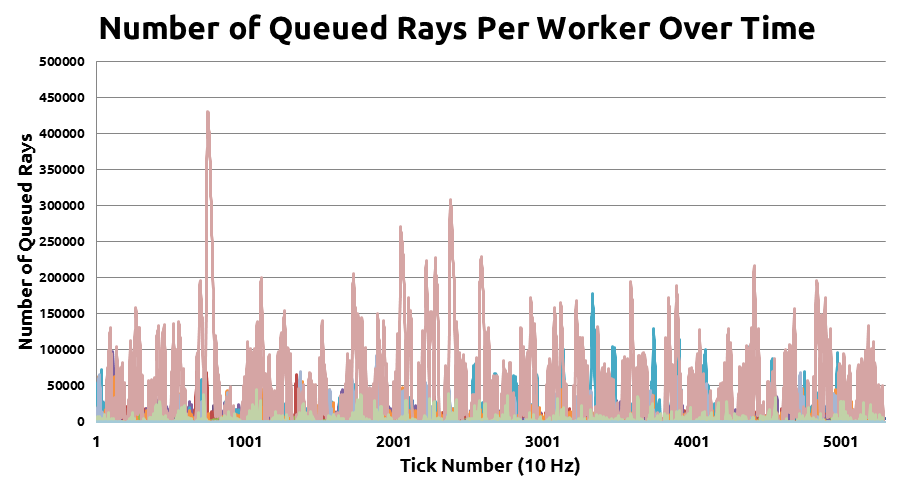
\includegraphics[width=140mm]{figures/queuesize.png}
    \captionfonts
    \caption{Number of rays queued on each worker over time. Different colors correspond to different workers.}
    \label{fig:queuesize}
\end{figure}

\begin{table}
\begin{center}
\begin{tabular}{|c||c|c|c|c|}
    \hline
    Worker & Average Queued & Max Queued & Max Storage & Memory Occupancy \\
    \hline
    \hline
    1 & 107 & 12221 & 1.49 MB & 0.04\% \\
    \hline
    2 & 506 & 29796 & 3.64 MB & 0.09\% \\
    \hline
    3 & 969 & 34970 & 4.27 MB & 0.10\% \\
    \hline
    4 & 3116 & 57597 & 7.03 MB & 0.17\% \\
    \hline
    5 & 1687 & 36981 & 4.51 MB & 0.11\% \\
    \hline
    6 & 1430 & 44053 & 5.38 MB & 0.13\% \\
    \hline
    7 & 4070 & 80899 & 9.88 MB & 0.24\% \\
    \hline
    8 & 2000 & 16861 & 2.06 MB & 0.05\% \\
    \hline
    9 & 3767 & 97429 & 11.89 MB & 0.29\% \\
    \hline
    10 & 7921 & 178191 & 21.75 MB & 0.53\% \\
    \hline
    11 & 4477 & 69702 & 8.51 MB & 0.21\% \\
    \hline
    12 & 4943 & 92043 & 11.24 MB & 0.27\% \\
    \hline
    13 & 51164 & 430736 & 52.58 MB & 1.28\% \\
    \hline
    14 & 2193 & 45428 & 5.55 MB & 0.14\% \\
    \hline
    15 & 0 & 0 & 0 MB & 0.00\% \\
    \hline
    16 & 18 & 1374 & 0.17 MB & 0.01\% \\
    \hline
\end{tabular}
\caption{Size of ray queues when rendering Toy Store with a 16-worker FlexRender cluster.}
\label{tb:rayqueues}
\end{center}
\end{table}

\section{Cluster Size}
\label{clustersize}

\textbf{TODO: commentary}

\textbf{TODO: cluster size table}

\chapter{Future Work}
\label{futurework}

Given that FlexRender is a relatively radical reimagining of ray tracer
architecture, the opportunities for improvement are vast. In this section we
document larger issues we noticed during implementation and testing that
could potentially offer significantly better results.

\section{System Optimizations}
\label{optimizations}

We present several potential optimizations. In Section \ref{networkhop} we
discuss a potential method to deter or eliminate the extra network hops in BVH
traversal, and in Section \ref{concerns} we discuss some underlying issues that,
if addressed, would yield better geometry distribution and parallelism.

\subsection{Eliminating Extra Network Hops}
\label{networkhop}

The first extra network hop occurs when rays are generated on machines that
control geometry they do not intersect with. This requires at least one
network hop before the ray could potentially intersect and be shaded. By performing
a prepass step before rendering began, we could gather information about the
layout of the scene in image space. By carefully choosing the slices of the
image that workers were responsible for casting primary rays in, we could
dramatically increase the chances that the ray would intersect the geometry
on the worker and finish shading without ever touching the network.

The second extra network hop occurs at the end of traversal, when the ray finishes
traversing the top-level BVH but ends up on a worker that is not the point of
intersection. Because the worker has no shading assets for that geometry, it
must pass the ray back to the ``winning" worker for shading. By distributing
all of the shading assets (shaders, textures, and materials) to all workers,
any worker would be capable of shading a ray at the conclusion of its BVH traversal.
This is possible because the rays carry along local geometry (mainly the surface
normal) from the point of closest intersection.

\subsection{Competing Concerns}
\label{concerns}

Currently there are two competing concerns in FlexRender. The first is to
distribute the scene data well, such that the geometry distribution is balanced
and everything is in-core. The second is to ``keep the chips hot", or maximize
the utilization of the available processing power in the cluster. Unfortunately,
these concerns are somewhat at odds at the moment. Good geometry distribution
is a result of distributing 3D space well, whereas good workload distribution
is a result of distributing screen space well. It is not immediately clear if
these two competing concerns can be addressed by a single renderer, but we
believe significant improvements could be made to both the geometry distribution
and the workload distribution that would significantly improve the state of affairs.

In retrospect, we believe that the Morton coding and Z-order curve was
a poor choice for the distribution of geometry. It was initially chosen because
we did not want to require a preprocessing (or \emph{baking}) step for
determining the optimal distribution of geometry. Since the scene was presumably
too large to fit in core on any one machine, preprocessing the scene as a whole
was deemed to be against the spirit of the problem.

The Z-order curve works well for spatially uniform scenes, but unfortunately a
lot of scenes that are interesting to render are usually uniformly distributed
in image space, not 3D space. The leads to a lot of degenerate scenes that
perform suboptimally when rendered with FlexRender. There would be a lot more
opportunities for distributing geometry in a more intelligent way if a
preprocessing step was allowed.

Secondly, the workload of rendering a particular piece of geometry falls on
the machine who is responsible for that geometry. This means that if a single
piece of geometry takes up a large portion of screen space, it will end up
being the bottleneck in rendering. Conversely, workers that hold geometry that
takes up very little screen space could end up contributing very little
horsepower to the render.

As mentioned in Section \ref{networkhop}, it is possible that a quick prepass
rendering could help alleviate this problem. If we have information about the
layout of the scene in image space prior to rendering, we have some opportunities
for moving things around to adjust the workload before it becomes a problem during
rendering. It is also possible that additional statisics monitoring could provide
on-the-fly migration of scene data to less loaded workers, although that would
require at least partially rebuilding the acceleration structure.

\section{Memory Optimizations}
\label{memory}

Based on the profiling results of our current implementation, the main
bottleneck is standard library calls and memory allocation. The transient
nature of many fixed-size fat rays is a perfect opportunity to use an object
pool to reduce allocation overhead and heap fragmentation.

In addition, the linear BVH nodes structures were intentionally padded to
64-bytes to match the cache line size on current CPUs. However without a custom
STL allocator for the vector that stores this array of nodes, cache alignment
is not guaranteed.

Lastly, there are a few places where the size of fat rays could be reduced.
For example, rather than storing the target position of an expected
intersection, the expected t value along the ray could be stored instead. This
would save 8 bytes. Another 4 bytes could be saved by removing the ``workers
touched" benchmarking field. By careful overlapping of mutually exclusive data
using unions, the size could probably be reduced further. Ideally a fat ray
would fit on a single cache line and the same aligned allocation strategy could
be applied to fat rays as well.

\section{GPGPU and Heterogeneous Architectures}
\label{hetergenous}

One of FlexRender's strengths is that it decouples the ray tracing computations
at the level of the individual ray. Because workers in the cluster speak a
defined network protocol to pass rays around, this opens the door for workers to
join the cluster with new and interesting machine architectures.

For example, consider general purpose GPU (GPGPU) computing. Vast speedups can
be attained by moving number-crunching operations to the GPU, but the CPU and
GPU usually exist in separate memory spaces. This means the memory transfer cost
of pushing data over the bus to the GPU must be amortized by the amount of
computation done on the GPU.

Because workers are never waiting on other workers for the results of a
computation, this opens up the possibility for batching data to a GPU worker.
Consider a worker who simply queues messages until enough are present to move
the data to the the GPU. FlexRender's architecture is amiable to amortizing
the cost of bus transfers in GPGPU computing.

\clearpage
\bibliography{flexrender}
\bibliographystyle{plain}
%\addcontentsline{toc}{chapter}{Bibliography}

\section*{Image Results}

\textbf{TODO: assorted renders}

\end{document} much faster 
